% I seguenti commenti speciali impostano:
% 1. 
% 2. PDFLaTeX come motore di composizione;
% 3. tesi.tex come documento principale;
% 4. il controllo ortografico italiano per l'editor.

% !TEX encoding = UTF-8
% !TEX TS-program = pdflatex
% !TEX root = tesi.tex
% !TEX spellcheck = it-IT
%!TEX program = xelatex
\documentclass[11pt,                    % corpo del font principale
    a4paper,                 % carta A4
    twoside,                 % impagina per fronte-retro
    openright,               % inizio capitoli a destra
    english,
    ctexart,
]{book}

%**************************************************************
% Importazione package
%************************************************************** 
%\usepackage{amsmath,amssymb,amsthm}    % matematica
\usepackage[UTF8]{ctex}
\usepackage[T1]{fontenc}                % codifica dei font:
% NOTA BENE! richiede una distribuzione *completa* di LaTeX

\usepackage[utf8]{inputenc}             % codifica di input; anche [latin1] va bene
% NOTA BENE! va accordata con le preferenze dell'editor

\usepackage[english]{babel}    % per scrivere in italiano e in inglese;
% l'ultima lingua (l'italiano) risulta predefinita

\usepackage{bookmark}                   % segnalibri

\usepackage{caption}                    % didascalie

\usepackage{chngpage,calc}              % centra il frontespizio

\usepackage{csquotes}                   % gestisce automaticamente i caratteri (")

\usepackage{emptypage}                  % pagine vuote senza testatina e piede di pagina

\usepackage{epigraph}            % per epigrafi

\usepackage{eurosym}                    % simbolo dell'euro

%\usepackage{indentfirst}               % rientra il primo paragrafo di ogni sezione

\usepackage{graphicx}                   % immagini

\usepackage{hyperref}                   % collegamenti ipertestuali

\usepackage[binding=5mm]{layaureo}      % margini ottimizzati per l'A4; rilegatura di 5 mm


\usepackage{microtype}                  % microtipografia

\usepackage{mparhack,fixltx2e,relsize}  % finezze tipografiche

\usepackage{nameref}                    % visualizza nome dei riferimenti                                      

\usepackage[font=small]{quoting}        % citazioni

%\usepackage{subfig}                     % sottofigure, sottotabelle

\usepackage[english]{varioref}          % riferimenti completi della pagina

\usepackage[dvipsnames]{xcolor}         % colori
\usepackage{formattazione}

\usepackage{booktabs}                   % tabelle                                       
\usepackage{tabularx}                   % tabelle di larghezza prefissata                                    
\usepackage{longtable}                  % tabelle su più pagine                                        
\usepackage{ltxtable}                   % tabelle su più pagine e adattabili in larghezza

\usepackage[toc, acronym]{glossaries}   % glossario
% per includerlo nel documento bisogna:
% 1. compilare una prima volta tesi.tex;
% 2. eseguire: makeindex -s tesi.ist -t tesi.glg -o tesi.gls tesi.glo
% 3. eseguire: makeindex -s tesi.ist -t tesi.alg -o tesi.acr tesi.acn
% 4. compilare due volte tesi.tex.
\usepackage[backend=biber,style=numeric-comp,hyperref,backref]{biblatex}
% eccellente pacchetto per la bibliografia;
% produce uno stile di citazione autore-anno;
% lo stile "numeric-comp" produce riferimenti numerici
% per includerlo nel documento bisogna:
% 1. compilare una prima volta tesi.tex;
% 2. eseguire: biber tesi
% 3. compilare ancora tesi.tex.

%**************************************************************
% file contenente le impostazioni della tesi
%**************************************************************

%**************************************************************
% Frontespizio
%**************************************************************

% Autore
\newcommand{\myName}{Giuseppe Boezio}
\newcommand{\myTitle}{Labeled Prolog: a computational model in 2p-KT}

% Tipo di tesi                   
\newcommand{\myDegree}{Master degree thesis}

% Università             
\newcommand{\myUni}{Alma Mater Studiorum - University of Bologna}

% Facoltà       
\newcommand{\myFaculty}{Artificial Intelligence}

% Dipartimento
\newcommand{\myDepartment}{Computer Science and Engineering - DISI}

% Titolo del relatore
\newcommand{\profTitle}{Prof.}

% Relatore
\newcommand{\myProf}{Roberta Calegari}

% Luogo
\newcommand{\myLocation}{Bologna}

% Anno accademico
\newcommand{\myAA}{2021-2022}

% Data discussione
\newcommand{\myTime}{03 February 2023}


\addto\captionsenglish{\renewcommand{\lstlistingname}{Code}}

%**************************************************************
% Impostazioni di impaginazione
% see: http://wwwcdf.pd.infn.it/AppuntiLinux/a2547.htm
%**************************************************************

\setlength{\parindent}{14pt}   % larghezza rientro della prima riga
\setlength{\parskip}{0pt}   % distanza tra i paragrafi


%**************************************************************
% Impostazioni di biblatex
%**************************************************************
\bibliography{bibliografia} % database di biblatex 

\defbibheading{bibliography} {
    \cleardoublepage
    \phantomsection 
    %\addcontentsline{toc}{chapter}{\bibname}
    \chapter*{\bibname\markboth{\bibname}{\bibname}}
}

\setlength\bibitemsep{1.5\itemsep} % spazio tra entry

\DeclareBibliographyCategory{opere}
\DeclareBibliographyCategory{web}

\addtocategory{opere}{womak:lean-thinking}
\addtocategory{web}{site:agile-manifesto}

\defbibheading{opere}{\section*{Bibliography}}
\defbibheading{web}{\section*{Websites}}


%**************************************************************
% Impostazioni di caption
%**************************************************************
\captionsetup{
    tableposition=top,
    figureposition=bottom,
    font=small,
    format=hang,
    labelfont=bf
}

%**************************************************************
% Impostazioni di glossaries
%**************************************************************
\input{Glossario} % database di termini
\makeglossaries


%**************************************************************
% Impostazioni di graphicx
%**************************************************************
\graphicspath{{images/}} % cartella dove sono riposte le immagini


%**************************************************************
% Impostazioni di hyperref
%**************************************************************
\hypersetup{
    %hyperfootnotes=false,
    %pdfpagelabels,
    %draft,	% = elimina tutti i link (utile per stampe in bianco e nero)
    colorlinks=true,
    linktocpage=true,
    pdfstartpage=1,
    pdfstartview=FitV,
    % decommenta la riga seguente per avere link in nero (per esempio per la stampa in bianco e nero)
    %colorlinks=false, linktocpage=false, pdfborder={0 0 0}, pdfstartpage=1, pdfstartview=FitV,
    breaklinks=true,
    pdfpagemode=UseNone,
    pageanchor=true,
    pdfpagemode=UseOutlines,
    plainpages=false,
    bookmarksnumbered,
    bookmarksopen=true,
    bookmarksopenlevel=1,
    hypertexnames=true,
    pdfhighlight=/O,
    %nesting=true,
    %frenchlinks,
    urlcolor=webbrown,
    linkcolor=RoyalBlue,
    citecolor=webgreen,
    %pagecolor=RoyalBlue,
    %urlcolor=Black, linkcolor=Black, citecolor=Black, %pagecolor=Black,
    pdftitle={\myTitle},
    pdfauthor={\textcopyright\ \myName, \myUni, \myFaculty},
    pdfsubject={},
    pdfkeywords={},
    pdfcreator={pdfLaTeX},
    pdfproducer={LaTeX}
}

%**************************************************************
% Impostazioni di listings
%**************************************************************
\lstset{
    language=[LaTeX]Tex,%C++,
    keywordstyle=\color{RoyalBlue}, %\bfseries,
    basicstyle=\small\ttfamily,
    %identifierstyle=\color{NavyBlue},
    commentstyle=\color{Green}\ttfamily,
    stringstyle=\rmfamily,
    numbers=none, %left,%
    numberstyle=\scriptsize, %\tiny
    stepnumber=5,
    numbersep=8pt,
    showstringspaces=false,
    breaklines=true,
    frameround=ftff,
    frame=single
} 


%**************************************************************
% Impostazioni di xcolor
%**************************************************************
\definecolor{webgreen}{rgb}{0,.5,0}
\definecolor{webbrown}{rgb}{.6,0,0}
\usepackage{chngcntr}
\counterwithout{footnote}{chapter}

%**************************************************************
% Altro
%**************************************************************

\newcommand{\omissis}{[\dots\negthinspace]} % produce [...]

% eccezioni all'algoritmo di sillabazione
\hyphenation
{
    ma-cro-istru-zio-ne
    gi-ral-din
}

\newcommand{\sectionname}{Section}
\addto\captions{\renewcommand{\figurename}{Figure}
                       \renewcommand{\tablename}{Table}}

\newcommand{\glsfirstoccur}{\ap{{[g]}}}

\newcommand{\intro}[1]{\emph{\textsf{#1}}}

%**************************************************************
% Environment per ``namespace description''
%**************************************************************

\newenvironment{namespacedesc}{
    \vspace{10pt}
    \par \noindent                              % start new paragraph
    \begin{description} 
}{
    \end{description}
    \medskip
}

\newcommand{\classdesc}[2]{\item[\textbf{#1:}] #2}
\renewcommand{\labelitemi}{$\bullet$}
\renewcommand{\labelitemii}{$\circ$}
\renewcommand{\labelitemiii}{-}
\renewcommand{\labelitemiv}{$\cdot$}
                     % file con le impostazioni personali
\raggedbottom
\begin{document}
    %**************************************************************
    % Materiale iniziale
    %**************************************************************
    \frontmatter
    % !TEX encoding = UTF-8
% !TEX TS-program = pdflatex
% !TEX root = ../tesi.tex

%**************************************************************
% Frontespizio 
%**************************************************************
\begin{titlepage}

\begin{center}

\begin{LARGE}
\textbf{\myUni}\\
\end{LARGE}

\vspace{10pt}

\begin{Large}
\textsc{\myDepartment}\\
\end{Large}

\vspace{10pt}

\begin{large}
\textsc{\myFaculty}\\
\end{large}

\vspace{220pt}
%\begin{figure}[htbp]
%\begin{center}
%%\includegraphics[height=6cm]{logo}
%\end{center}
%\end{figure}
%\vspace{30pt}

\begin{LARGE}
\begin{center}
\textbf{\myTitle}\\
\end{center}
\end{LARGE}

\vspace{10pt} 

\begin{large}
\textsl{\myDegree}\\
\end{large}

\vspace{20pt}

\begin{large}
\begin{flushleft}
\textit{Supervisor}\\
\vspace{5pt} 
\profTitle \myProf\\
\textit{Co-supervisor}\\
\vspace{5pt}
Prof. Giovanni Ciatto
\end{flushleft}

\vspace{0pt} 

\begin{flushright}
\textit{Candidate}\\
\vspace{5pt} 
\myName
\end{flushright}
\end{large}

\vspace{20pt}

\line(1, 0){338} \\
\begin{normalsize}
\textsc{Academic Year \myAA - Third session}
\end{normalsize}

\end{center}
\end{titlepage}
    % !TEX encoding = UTF-8
% !TEX TS-program = pdflatex
% !TEX root = ../tesi.tex

%**************************************************************
% Colophon
%**************************************************************
\clearpage
\phantomsection
\thispagestyle{empty}

\hfill

\vfill

\noindent\myName: \textit{\myTitle,}
\myDegree,
\textcopyright\ \myTime.

\cleardoublepage
    % !TEX encoding = UTF-8
% !TEX TS-program = pdflatex
% !TEX root = ../tesi.tex

%**************************************************************
% Sommario
%**************************************************************
\cleardoublepage
\phantomsection
\pdfbookmark{Abstract}{Abstract}
\begingroup
\let\clearpage\relax
\let\cleardoublepage\relax
\let\cleardoublepage\relax

\chapter*{Abstract}

%\vfill
%
%\selectlanguage{english}
%\pdfbookmark{Abstract}{Abstract}
%\chapter*{Abstract}
%
%\selectlanguage{italian}
2P-Kt is an interpreter for Prolog language which is written in a way such that it can be easily extended and customized to deal with
specific needs. In the current scenario Constraint Logic Programming (CLP) has been supported by this system using an interface which is
as close as possible to the predicates' signatures used by famous and most used CLP(X) family of libraries supported by SWI Prolog interpreter.
A real case study concerning school timetabling is described to show a practical usage of CLP(FD) library implemented with the aforementioned 2P-Kt interpreter.
This case study shows how libraries have been modularized in such a way that they can be used as dependencies in every project developed for the Java
Virtual Machine (JVM).\newline
Constraint Logic Programming represents only a particular scenario for logic programming: for this reason a framework which extends the
mechanism of Labelled Variables has been implemented to show how it is possible to frame all variations and extensions of logic programming under a
single language reducing the huge amount of existing languages and libriaries and focusing on more on how to manage different domain needs using labels
which can be associated to every kind of term.
\endgroup

\vfill


    % !TEX encoding = UTF-8
% !TEX TS-program = pdflatex
% !TEX root = ../tesi.tex

%**************************************************************
% Ringraziamenti
%**************************************************************
\cleardoublepage
\phantomsection
\pdfbookmark{Acknowledgements}{Acknowledgements}


%\bigskip

\begingroup
\let\clearpage\relax
\let\cleardoublepage\relax
\let\cleardoublepage\relax

\chapter*{Acknowledgements}

\noindent First, I would like to express my deepest gratitude to Professor Calegari and Professor Ciatto for all the support they provided me during the internship and thesis redaction processes.\\

\noindent Second, I would like to thank my family, my friends and all people who believed in me during this long study path.\\


\noindent Last but not least, I would like to thank myself to have been able to never give up during these two years. \\

\noindent\textit{\myLocation, \myTime}
\hfill \myName

\endgroup


    % !TEX encoding = UTF-8
% !TEX TS-program = pdflatex
% !TEX root = ../tesi.tex

%**************************************************************
% Indici
%**************************************************************
\cleardoublepage
\pdfbookmark{\contentsname}{tableofcontents}
\setcounter{tocdepth}{2}
\tableofcontents
%\markboth{\contentsname}{\contentsname} 
\clearpage

\begingroup 
    \let\clearpage\relax
    \let\cleardoublepage\relax
    \let\cleardoublepage\relax
    %*******************************************************
    % Elenco delle figure
    %*******************************************************    
    \phantomsection
    \pdfbookmark{\listfigurename}{lof}
    \listoffigures

    \vspace{8cm}

    %*******************************************************
    % Elenco delle tabelle
    %*******************************************************
    \phantomsection
    \pdfbookmark{\listtablename}{lot}
    \listoftables
    \vspace*{8ex}
\endgroup

\cleardoublepage

    \cleardoublepage

    %**************************************************************
    % Materiale principale
    %**************************************************************
    \mainmatter
    % !TEX encoding = UTF-8
% !TEX TS-program = pdflatex
% !TEX root = ../tesi.tex

%**************************************************************
\chapter{Introduction}\label{ch:introduction}
%**************************************************************

\intro{In this section we will present the summarized content of the whole thesis.}
%\noindent Esempio di utilizzo di un termine nel glossario \\
%\gls{api}. \\
%
%\noindent Esempio di citazione in linea \\
%\cite{site:agile-manifesto}. \\
%
%\noindent Esempio di citazione nel pie' di pagina \\
%citazione\footcite{womak:lean-thinking} \\

%**************************************************************

\section{Background}\label{sec:background}
Computer vision (CV) is a field of artificial intelligence that deals with the study of how computers can be made to gain high-level understanding from digital images or videos.
If AI allows the computer to think like a human as well as computer vision allows the computer to see like a human.

CV works like the human visual system, with the big difference in the fact that human uses year and year of experience to help the mind to understand what it is seeing.
As the biological neurons processes the information in the brain, the artificial neurons processes the information in the artificial neural network following the Hebbian plasticity (\cite{site:hebbian-plasticity}) rule: the connection between two neurons is strengthened if they are active at the same time.

In recent years, deep learning has revolutionized the CV field, achieving excellent results in many tasks, like: image classification, object detection, semantic segmentation, image captioning, image generation, etc.

The image classification task consists of assigning a label to an image with only one object (\hyperref[fig:figure-tulips]{Figure 1.1}).
\begin{figure}[H]
    \centering
    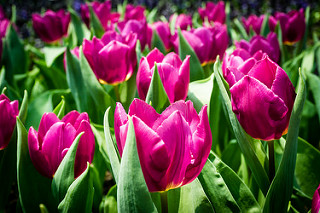
\includegraphics[width=0.8\textwidth]{images/1_1_tulips}
    \caption[Example of image classification]{Image classification: this image is classified as a tulip}
    \label{fig:figure-tulips}
\end{figure}
The object detection tasks consists of assigning a label and a bounding box to each object in the image.
The bounding box is a rectangle that encloses the object(\hyperref[fig:figure-object-detection]{Figure 1.2}).
\begin{figure}[H]
    \centering
    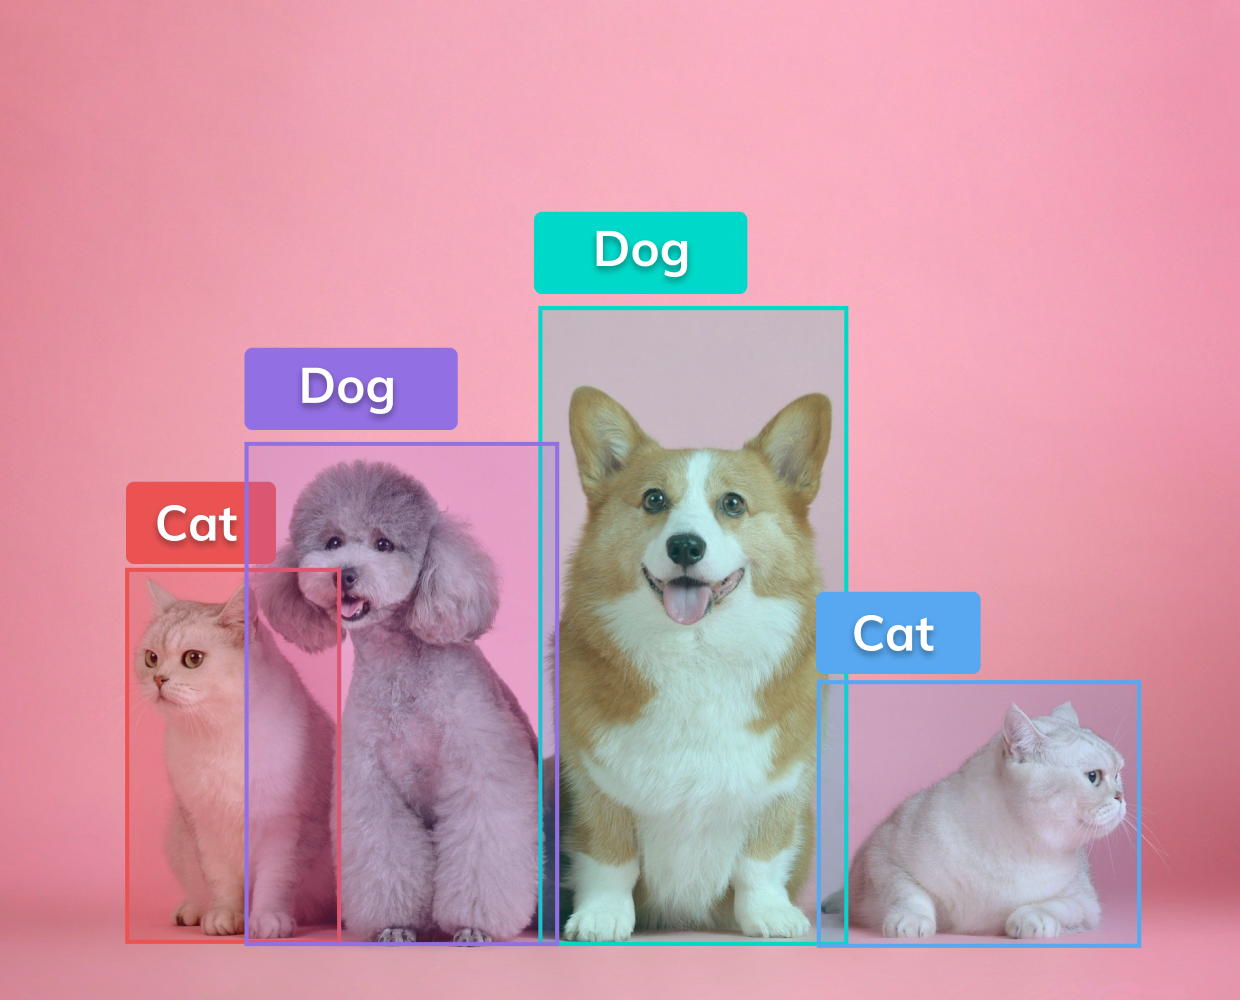
\includegraphics[width=0.8\textwidth]{images/1_1_object_detection}
    \caption[Example of object detection]{Object detection: this image contains two classes of objects, cat and dog.}
    \label{fig:figure-object-detection}
\end{figure}
The semantic segmentation task consists of assigning a label to each pixel of the image(\hyperref[fig:figure-semantic-segmentation]{Figure 1.3}).

\begin{figure}[H]
    \centering
    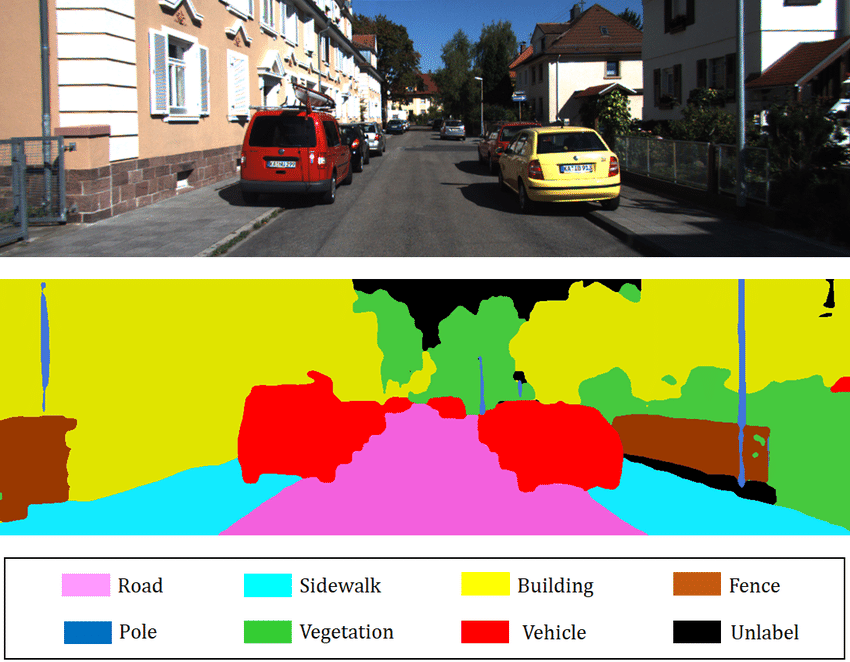
\includegraphics[width=0.8\textwidth]{images/1_1_semantic_segmentation}
    \caption[Example of semantic segmentation]{Semantic segmentation: each pixel is assigned a label.}
    \label{fig:figure-semantic-segmentation}
\end{figure}

Then, the modern CV systems can be used not only on the images, but also on video, like surveillance cameras to perform the real-time object detection and tracking, the most famous model is YOLOv3 (Redmon et al.~\cite{yolov3_paper}) (\hyperref[fig:figure-yolo-v3]{Figure 1.4}).

\begin{figure}[H]
    \centering
    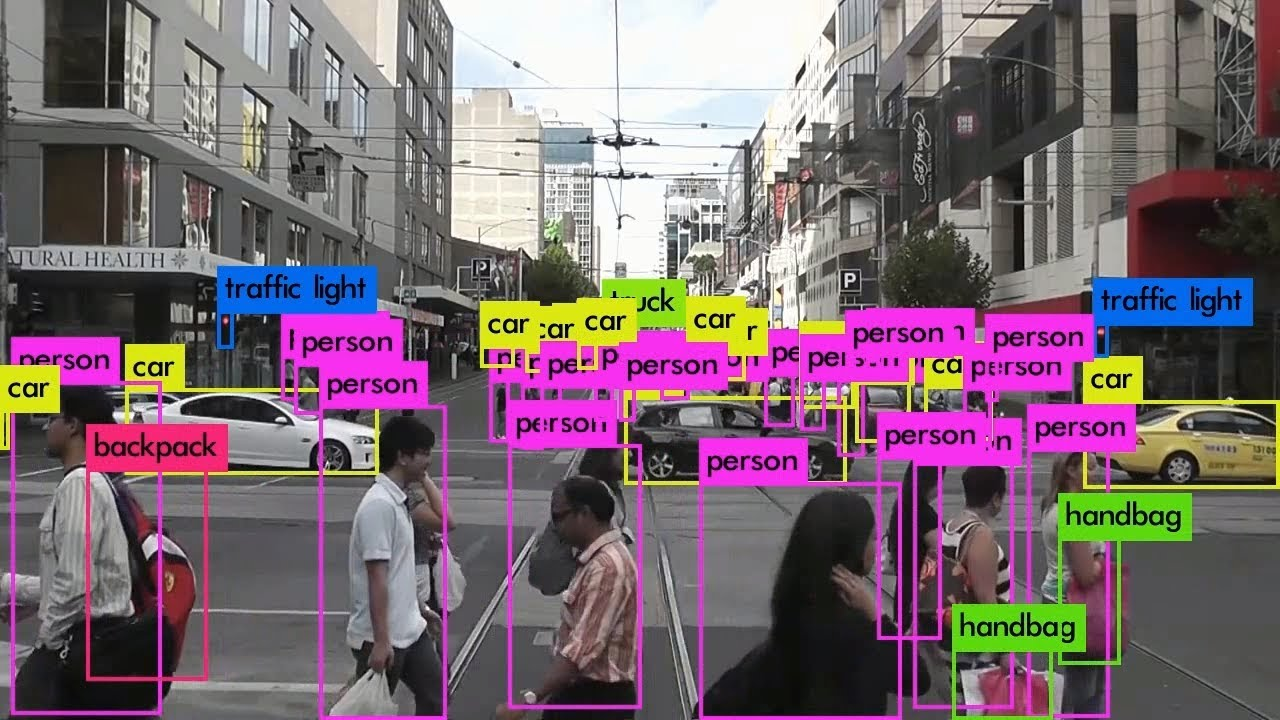
\includegraphics[width=0.8\textwidth]{images/1_1_yolov3}
    \caption{YOLO-V3 in action.}
    \label{fig:figure-yolo-v3}
\end{figure}



%**************************************************************

\section{Problem}\label{sec:problem}
The term "odometry" originated from two Greek works \emph{hodos} (meaning "journery" or "travel") and \emph{metron} (meaning "measure").
This derivation is related to the estimation of the change in a robot's pose (translation and rotation) over time.
Mobile robot use data from motion sensor to estimate their position relative to their initial location, this is called odometry.
VO is a technique used to localize a robot by using only a stream of images acquired from a single or multiple camera.
There are different ways to classify the typology of Visual Odometry:
\begin{itemize}
    \item based on the camera setup:
        \begin{itemize}
            \item Monocular VO: using only one camera;
            \item Stereo VO: using two cameras;
        \end{itemize}
    \item based on the information:
        \begin{itemize}
            \item Feature based method: which extracts the image feature points and tracks them in the image sequence;
            \item Direct method: a novel method which uses the pixel intensity in the image sequence directly as visual input.
            \item Hybrid method: which combines the two methods.
        \end{itemize}
    \item Visual inertial odometry: if a \gls{imu} is used within the VO system, it is commonly referred to as Visual inertial odometry.
\end{itemize}
We can represent the pose in different ways, for example: \textbf{euler angles}, \textbf{quaternions}, \textbf{rotation matrices} combined with \textbf{translation vectors}.

The goal is to create a \gls{nn}, using a \textbf{ResNet} to extract features from images and the \textbf{transformer} presented by Vaswani et al.~(\cite{transformer_paper}), which is able to estimate a sequence of camera poses given a sequence of images.

%**************************************************************

\section{Why transformer?}\label{sec:why-transformer}

We think that the transformer is a good candidate to solve the problem of visual odometry because it is able to learn a sequence from one domain and translate it into another sequence from another domain.
This kind of task is called sequence-to-sequence translation, e.g., machine translation.

Traditionally, this task is tackled by using recurrent neural networks (RNNs), but they have some limitations, such as the vanishing gradient problem, which makes them difficult to train.

Other VO approaches uses the CNNs, but in CNNs the features are statically weighted using pretrained weights, while in the transformer the features are dynamically weighted based on the context and receptive fields of CNNs can be limiting the performance of the whole network.
The success of the CNN derives from the fact the shared weights explicitly encode how specific identical patterns are repeated in images, this ensures the convergence also in relatively small dataset, but also limits the modelling capacity.
Meaning that CNNs can converge to a good performance also with a relatively small dataset.

Meanwhile, the vision transformers do not enforce such strict bias, so, transformer has the higher learning capacity, but it's harder to train.

So, given the high learning capacity of the transformer, its capability to adapt to various tasks and its good ability in seq2seq translation, we think that it is a good candidate to solve the problem of visual odometry.


%**************************************************************

%! Author = wxw85
%! Date = 01/08/2022

\section{Solution}\label{sec:solution}
%**************************************************************

We tried to tackle the problem by designing a deep neural network which is composed by a feature extractor, the transformer and a MLP to predict the pose.
We feed the feature extractor with a sequence of images, we tried both grey-scale and RGB images, in this way, we obtain a sequence of embeddings (both size 512 and 2048), the embedding are then fed into the transformer (both encoder-only and encoder-decoder version) and the output of the transformer is fed into the MLP to predict the sequence of poses.

\begin{figure}[H]
    \centering
    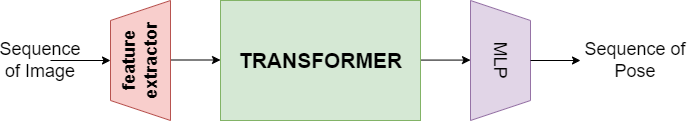
\includegraphics[width=0.8\textwidth]{images/1_4_general_solution}
    \caption{General representation of the model.}
    \label{fig:figure-1_4_solution}
\end{figure}

We use a sequence of image because the transformer model, originally designed for the machine translation, it requires as input a sequence of embeddings, then it outputs another sequence of embeddings.
For major details about the transformer, we refer to \hyperref[sec:exp-models]{\S4.1 Experiments - Models} and \hyperref[sec:models]{\S5.3 Implementation - Models}.

%**************************************************************

\section{Thesis organization}\label{sec:thesis-organization}
\begin{description}
    \item[{\hyperref[ch:introduction]{First chapter}}] introduces the general content about thesis and gives a short presentation of the topic, the problem and the solution we propose;

    \item[{\hyperref[ch:theoretical-foundations]{Second chapter}}] a deepening about the theoretical foundations used during the stage and the project;

    \item[{\hyperref[ch:datasets]{Third chapter}}] presents the datasets used during for the training and the testing of the model;

    \item[{\hyperref[ch:experiments]{Fourth chapter}}] presents the experiments did during to develop the system;

    \item[{\hyperref[ch:implementations]{Fifth chapter}}] presents the different implementations of the system;

    \item[{\hyperref[ch:final-discussions]{Sixth chapter}}] discusses about the results and possible future developments.
\end{description}
During the drafting of the essay, following typography conventions are considered:
\begin{itemize}
    \item the acronyms, abbreviations, ambiguous terms or terms not in common use are defined in the glossary, in the end of the present document;
    \item the first occurrences of the terms in the glossary are highlighted like this: \gls{word};
    \item the terms from the foreign language or jargon are highlighted like this: \emph{italics}.
\end{itemize}

%**************************************************************


    % !TEX encoding = UTF-8
% !TEX TS-program = pdflatex
% !TEX root = ../tesi.tex

%**************************************************************

\chapter{Theoretical foundations}
\label{ch:theoretical-foundations}
%**************************************************************

\intro{In this chapter we will present the theoretical knowledge useful to understand the content from successive chapters.}\\

%**************************************************************

\section{Deep Learning}\label{sec:deep-learning}

Deep learning method is part of machine learning methods based on artificial neural network with representation learning.
The learning process can be supervised, semi-supervised, or unsupervised.

There is a very large variety of deep learning architectures, some of them are specialized in some fields meanwhile others have a broader usage, especially, there are CNNs and Transformers.

In recent years, the field of computer vision has been growing in complexity and the number of applications has been increasing, in addition to those presented in \hyperref[sec:background]{Section 1.1 Computer vision}, there are \gls{slam} and visual odometry which is a task in which the robot is able to understand where it is and how it is oriented.

The development of computer vision has been a long process, the growth is favoured by the development of new hardware components and new challenges, about the latters, we have
CIFAR-10 (Doon et al.~\cite{cifar10_paper}), Fashion-MNIST(Xiao et al.~\cite{fashion_mnist_paper}), MS-Coco (Lin et al.~\cite{ms_coco_paper}) and ImageNet (Deng et al.~\cite{imagenet_paper}).
These datasets are often used as benchmark for novel approaches.

For the architectures, starting from AlexNet (Krizhevsky et al.~\cite{alex_net_paper}), then VGG (Simonyan et al.~\cite{vgg_paper}), Inception-V1 (Szegedy et al.~\cite{inception_v1_paper}), Inception-V2 (Szegedy et al.~\cite{inception_v2_paper}), ResNet (He et al.~\cite{resnet_paper}), etc., the complexity of the models has increased enormously.
Each of these models introduced some innovations and improved the performance on the benchmarks, for example:
\begin{itemize}
    \item AlexNet introduced the concept of the \emph{convolutional neural network} (CNN) and use of the separation of the models into two different GPUs.
    \item VGG introduced the concept of stage, which repeated more times, composes the model.
    \item Inception-V1, Inception-V2 and Inception-V3 which are based on the concept of \emph{inception module} which was composed by different paths that the input has to go through to reach the output.
    \begin{figure}[H]
        \centering
        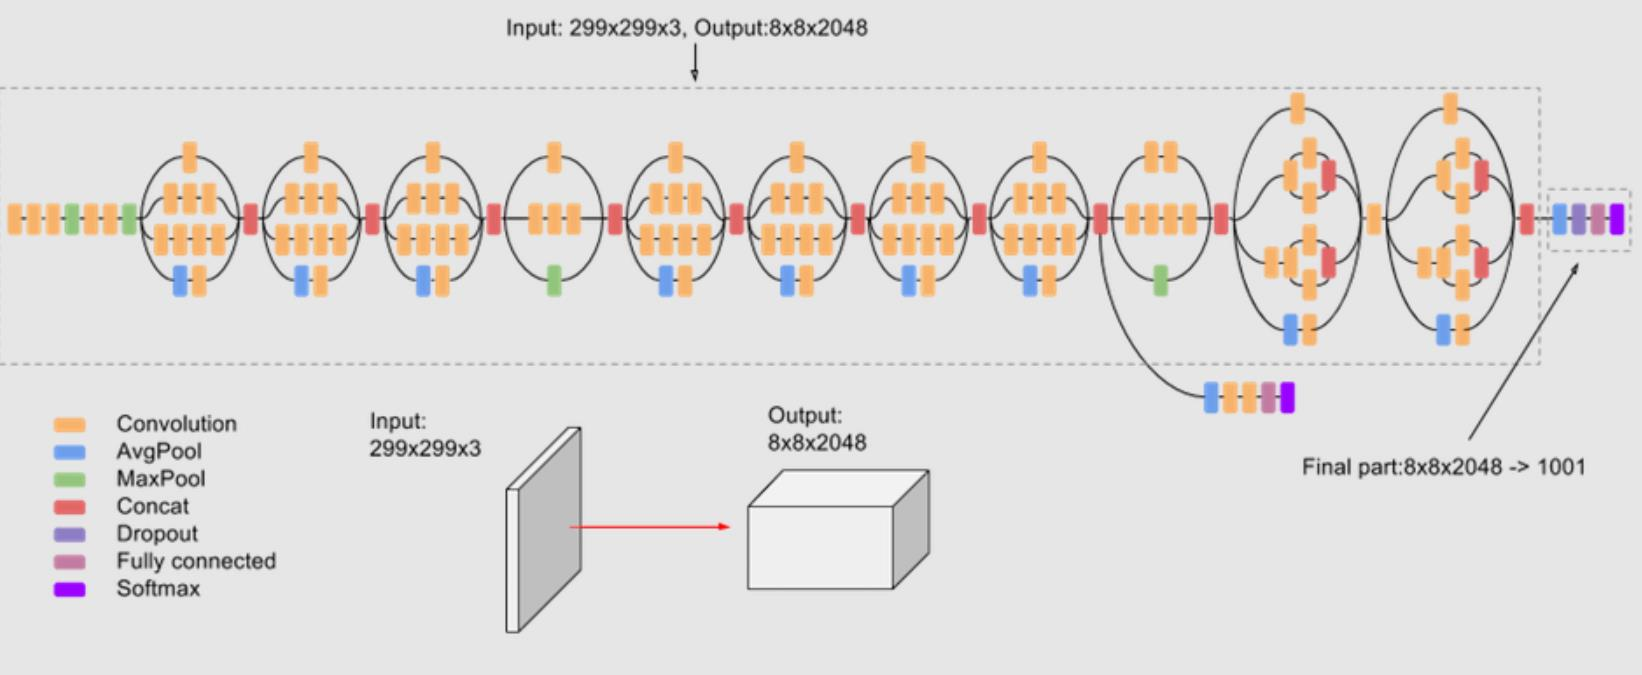
\includegraphics[width=\textwidth]{images/2_inception_v3}
        \caption{Inception V3 Structure.}\label{fig:inception-v3}
    \end{figure}
    \item ResNet is a model that is based on the concept of \emph{residual network} which is composed by several blocks of the same type with the skip connections:
    \begin{figure}[H]
        \centering
        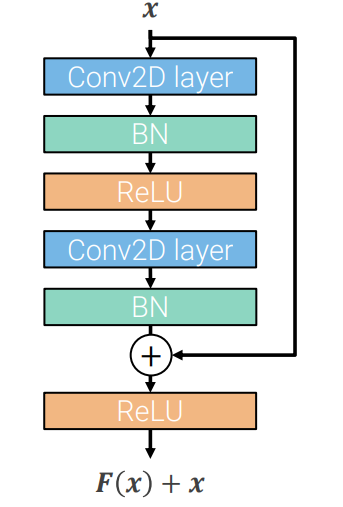
\includegraphics[width=0.4\textwidth]{images/2_1_skip_connection}
        \caption{Skip connection.}\label{fig:skip-connection}
    \end{figure}
    Basically, the input of the block is added to the output before feeding it to the next block, in this way, we can avoid the \gls{vanishing gradient problem} making easier the training process.
\end{itemize}
After this, the computer-visionists lend the Transformer architecture (Vaswani et al.~\cite{transformer_paper}) from \gls{nlp}, bringing up ViT (Dosovitskiy et al.~\cite{vit_paper}) which is based on the \gls{mha} mechanism.
A multi-head attention is a module of attention mechanisms repeated several times in parallel.
In this way, the model can attend to different parts of the input, forming the cross-attention over different parts of the input.
For major details, please refer to \hyperref[subsec:transformer]{\S2.1.2 Transformer}.


\subsection[CNN]{Convolutional Neural Network}\label{subsec:conv-neural-network}
The \gls{cnn} is a class of artificial neural network, it is used in almost every imagery related task, such as image classification, object detection, image segmentation, etc.

The CNN takes an input image, assign importance (learnable weights and biases) and process the input image by using the convolution operation extracting features.
There are two important parameters in the convolution operation, the kernel size and the stride.
The kernel is a matrix which is used to perform the convolution operation, the stride is the number of pixels the kernel slides each step over the input image to produce a new pixel of the output feature map.
With stride, we can control the size of the output image, if the stride is equal to 1, the output image will have the same size of the input image, if the stride is equal to 2, the output image will have half the size of the input image.
\begin{figure}[H]
    \centering
    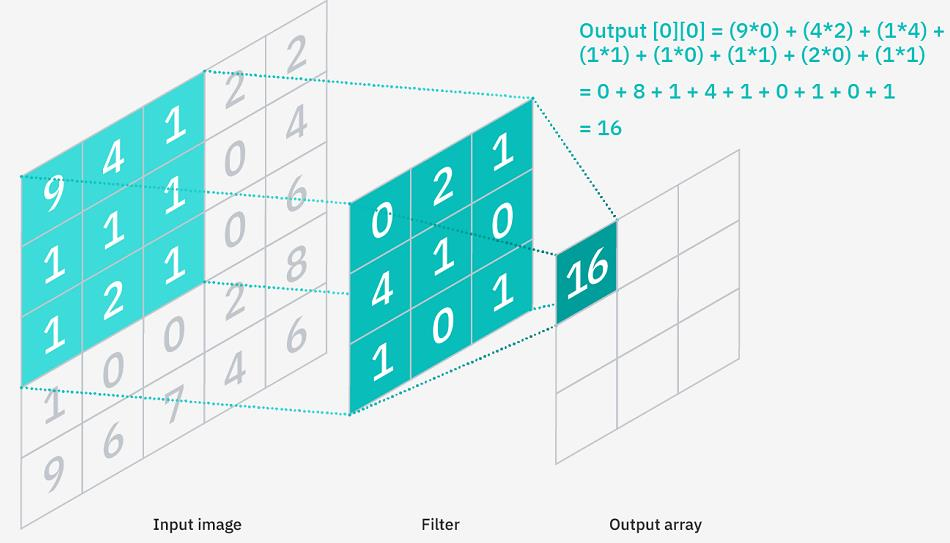
\includegraphics[width=\textwidth]{images/2_convolutions}
    \caption[Example of convolution]{Convolutions: every single element of the output feature map is obtained by summing the element-wise product between the elements from the input feature map and the kernel. The whole feature map is then obtained sliding the kernel over the input feature map.}
    \label{fig:figure-convolutions}
\end{figure}
Then, there are pooling layers, usually max-pooling and average pooling, which can reduce the dimensionality of the feature maps by setting strides $>=2$, which is useful to reduce the computational cost.
An important property of max-pooling is that it is translation invariant, which means that the output of the max-pooling layer is the same regardless of the position of the input feature map.
For example, max-pooling is computed as showed in the image:
\begin{figure}[H]
    \centering
    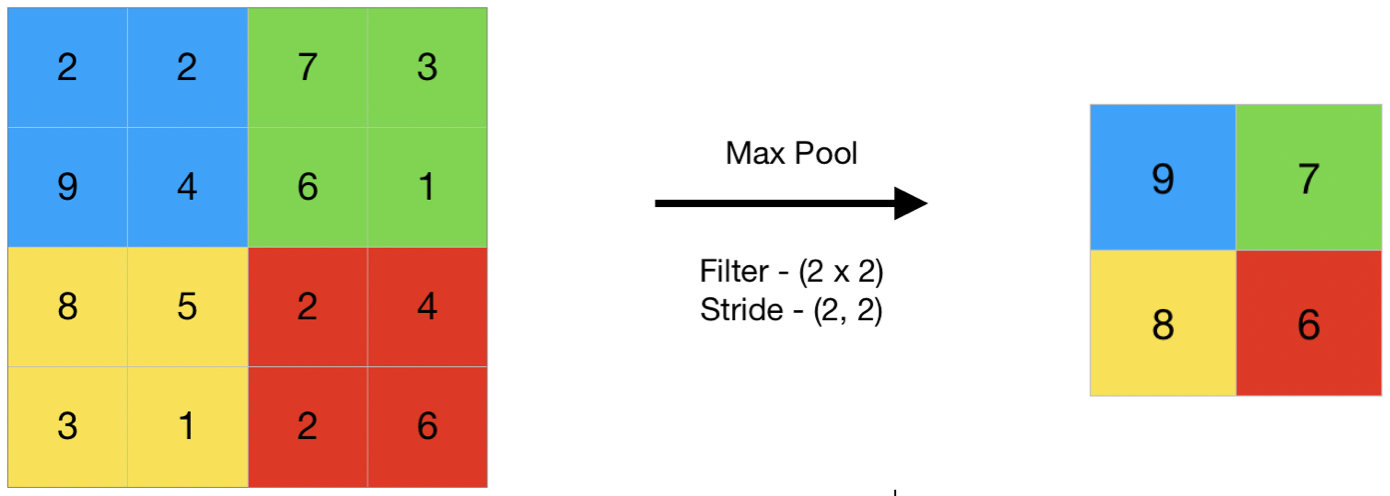
\includegraphics[width=\textwidth]{images/2_max_pooling}
    \caption[Example of max-pooling]{Max-pooling: essentially, it strides over the input image and takes the max value of the area covered by the kernel.}
    \label{fig:figure-max-pooling}
\end{figure}
With stride = 2, sliding over the input feature map and taking the maximum value of the window, the dimensionality of the feature map is reduced.

Another important component is the activation function, \gls{relu} is the most used one, it is defined as:
\begin{equation}
    ReLU(x) = \max(0, x)
    \label{eq:expression-relu}
\end{equation}
It guarantees the non-linearity of the network, allowing the network to learn more complex features.
These are the main components of a CNN, but there are other components, such as batch normalization and dropout which are used to improve the performance of the network reducing the over-fitting.
Increasing the number of layers and combining the pooling layers, the CNN is able to extract more and more complex features, such as edges, lines, shapes, etc.
Currently, the most used CNN architecture is the ResNet which will be used in the project as feature-extractor.

\subsection{Transformer}\label{subsec:transformer}
The transformer architecture is a class of neural network architecture, born for the task of machine translation, but it has been used in many vision tasks.

As introduced in ~\cite{transformer_paper}, the Transformer is a model architecture based entirely on attention mechanism.
Which can be divided into different steps: the first step of attention mechanism is to compute the Q, K and V vectors, by multiplying the input vector $x$ by the weight matrices $W_q$, $W_k$ and $W_v$.
Then, the attention weights are computed by using the scaled dot product attention, which is the softmax of the dot product between the query and the key vectors divided by the square root of the dimensionality of the key vector.
Finally, the attention weights are multiplied by the value vector to obtain the output vector.
The output vector is then passed through a feed-forward neural network, which is composed by two linear layers with ReLU activation function, added to the input vector and normalized by the layer normalization.
The self-attention module is then repeated $N$ times, where $N$ is the number of layers.

The whole process can be summarized as the:
\begin{equation}
    Attention(Q, K, V) = softmax\left(\frac{QK^T}{\sqrt{d_k}}\right)V
    \label{eq:expression-scaled-dot-product}
\end{equation}
And the graphical representation is:

\begin{figure}[H]
    \centering
    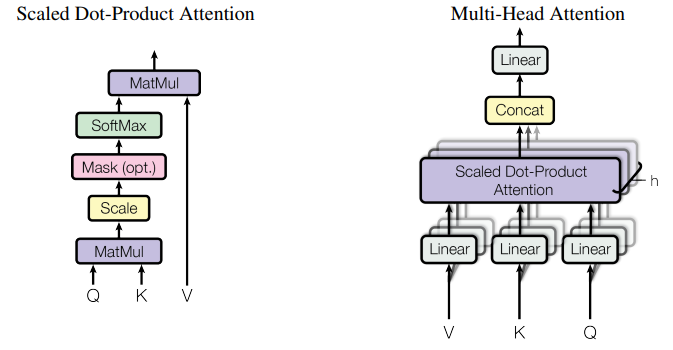
\includegraphics[width=\textwidth]{./images/2_attention}
    \caption[Attention mechanisms]{Attention mechanism: (Left) scaled-dot-product attention. (right) Multi-head attention which is obtained by combining many scaled-dot-product attention.}
    \label{fig:figure-encoder-structure}
\end{figure}

An important notion introduced is the multi-head attention, which is using more scaled dot product attention, each one with different weights, and concatenating each output vectors.
And this is the transformer encoder.

Then, using a slightly modified version of the self-attention module, we obtain the decoder, which takes as input also the output sequence from encoder, and repeating the number of encoder and decoder modules, we obtain the whole transformer architecture, as follows:

\begin{figure}[H]
    \centering
    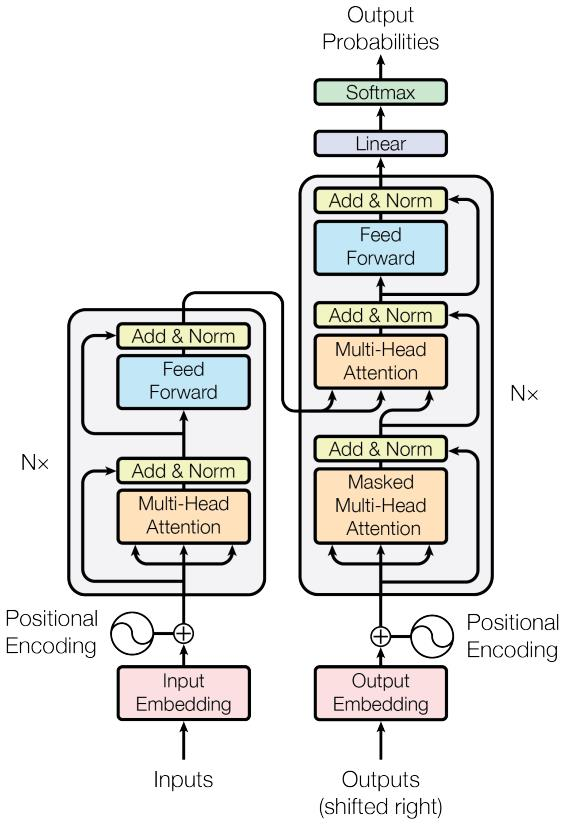
\includegraphics[width=0.7\textwidth]{./images/2_transformer}
    \caption[Transformer architecture]{Transformer architecture: the encoder and decoder modules are composed by a self-attention module and a feed-forward neural network repeated $N$ times.}
    \label{fig:figure-transformer-architecture}
\end{figure}

With this architecture the new state-of-the-art results have been achieved in Natural Language Processing, especially in machine translation (a \gls{seq2seq} task).
Then the adapted version applied to vision tasks also brought very good results, such as in object detection, image captioning, etc.

Another important notion is the mask which is used in sequence-to-sequence models, such as the transformer more specifically in the decoder, to avoid the model to attend to the future tokens.
To ensure this, the future positions are masked with $-\infty$ before the softmax step in the self-attention calculation.

%**************************************************************

\section{Odometry}\label{sec:visual-odometry}
As introduced in \hyperref[sec:the-problem]{\S1.2}, the problem of odometry is about the estimation of the change in a robot's pose over time.

The odometry, also known as self-localization, can be classified in different ways, in the next section, there is a more detailed description of the different types of odometry.

\subsection{Taxonomy}\label{subsec:tassonomy}
There different types of odometry, which based on the classification of Alkendi et al.~\cite{vo_state_of_art} can be divided into two main categories: \gls{gnss} available and GNSS not available.
\begin{figure}[H]
    \centering
    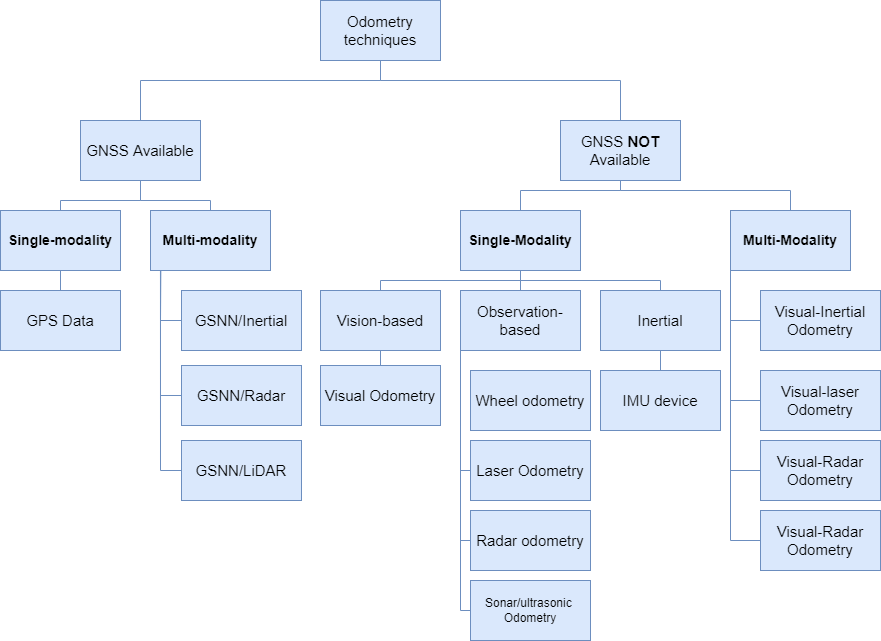
\includegraphics[width=\textwidth]{images/2_2_taxonomy_odometry}
    \caption{Taxonomy of odometry techniques.}\label{fig:odometry-taxonomy}
\end{figure}
The main difference between the left-branch and the right branch is that in the left one, the systems can use the Global Navigation Satellite System (GNSS) to get the position of the robot, while in the right one, the systems cannot use the GNSS, so the task is much more difficult.
Then, for the right branch, there are two classes, the first one is \textit{Single modality} meanwhile the other is about the combination of different modalities.
Finally, the \textit{Single modality} can be divided into three classes, the first one is \textit{Vision-based}, second one is \textit{Observation based} and the last is \textit{Inertial}.
The difference between first two are is that the first is about visual information, i.e., images, while the second one is about the information from the sensors, i.e., the laser scanner, radar sensor and sonar sensor.

The visual odometry, then, can be divided in many categories, like in the following figure.

\begin{figure}[H]
    \centering
    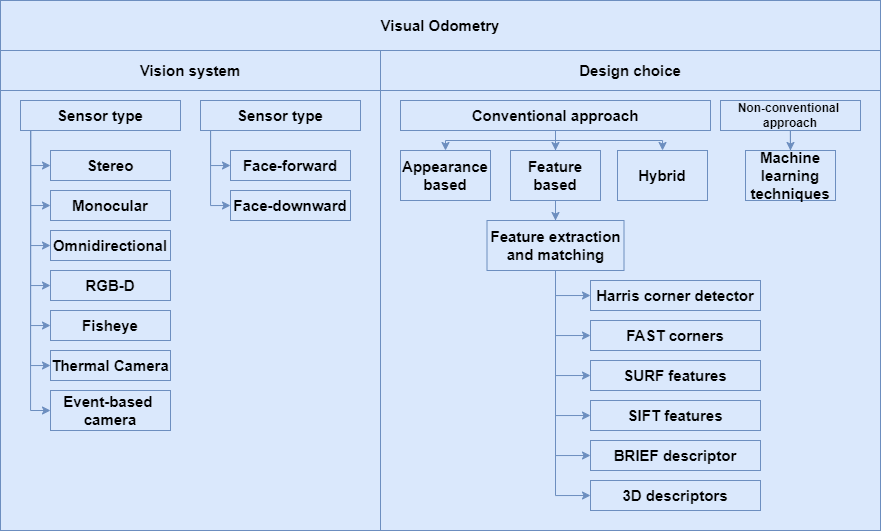
\includegraphics[width=\textwidth]{images/2_2_visual_odometry_taxonomy}
    \caption{Taxonomy of visual odometry techniques proposed in the literature.}\label{fig:visual-odometry-taxonomy}
\end{figure}
Our solution will be a monocular, face-forward, non-conventional approach by using machine learning technique, in particular, a neural network based on transformer model.

\subsection{Reference systems}\label{subsec:reference-systems}
To tackle the problem of odometry, we need to choose the representation system to adopt.
There are many way of representing the pose of the camera or the robot, but the most common are the \textit{Euler angles} and \textit{roto-translation matrix}.
The KITTI dataset provides the pose of the camera in the \textit{roto-transformation matrix} format flattened into a list of 12 numbers.

\subsubsection*{Euler angles}
The Euler angles (\cite{euler_angles}) are introduced by Euler to describe the orientation of a rigid body with respect to a fixed coordinate system.
According to Euler's rotation theorem, any rotation may be described using three angles.
If the rotations are written in terms of rotation matrices \textbf{D}, \textbf{C} and \textbf{B}, then, a general rotation \textbf{A} can be written as:
\begin{equation}
    \textbf{A} = \textbf{D} \textbf{C} \textbf{B}
    \label{eq:general_rotation}
\end{equation}
where $D$, $C$ and $B$ are called Euler angles.
There are several conventions for Euler Angles, depending on the axes about which the rotation are carried out.
Write the matrix \textbf{A} as:
\begin{equation}
    \textbf{A} = \begin{bmatrix}
                     a_{11} & a_{12} & a_{13} \\
                     a_{21} & a_{22} & a_{23} \\
                     a_{31} & a_{32} & a_{33}
    \end{bmatrix}
    \label{eq:matrix_A}
\end{equation}
The so-called ``x-convention'' is the most common one, in this convention, the rotation given by angles ($\phi$, $\theta$, $\psi$) respectively for \textit{roll}, \textit{pitch} and \textit{yaw} is defined as:
\begin{enumerate}
    \item by an angle $\phi$ about the $z$-axis using $D$;
    \item then, by an angle $\theta \in [0,\pi]$ about the former $x$-axis using $C$;
    \item third rotation is by an angle $\psi$ about the former $z$-axis using $B$.
\end{enumerate}
Here, we have a graphical example of the \textit{roll}, \textit{pitch} and \textit{yaw} axis:
\begin{figure}[H]
    \centering
    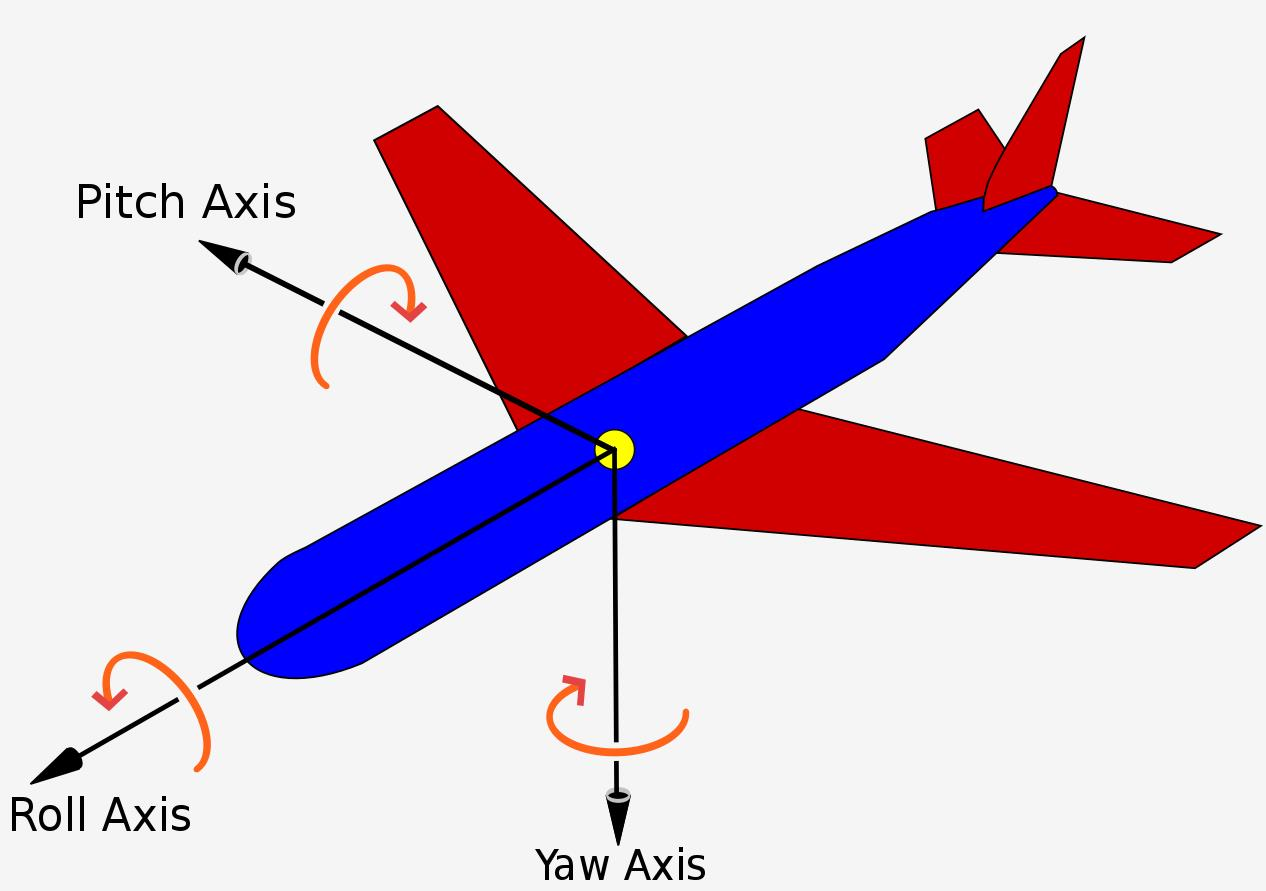
\includegraphics[width=0.6\textwidth]{images/2_2_roll_pitch_yaw}
    \caption{Roll-Pitch-Yaw axis representation.}\label{fig:euler-angles}
\end{figure}
So, by adding x, y, z axis as translations to three rotation angles ($\phi$, $\theta$, $\psi$) we can represent the pose of the camera in the world frame by using six numbers.
\subsubsection*{Roto-translation matrix}
In linear algebra, a \textit{roto-translation matrix} is a matrix that represents a rigid-body transformation.
It's called \textit{roto-translation} because it can be decomposed into a \textit{rotation matrix} and a \textit{translation}.

In details, the rotation matrix is defined as:
\begin{equation}
    \textbf{R} = \begin{bmatrix}
                     r_{11} & r_{12} & r_{13} \\
                     r_{21} & r_{22} & r_{23} \\
                     r_{31} & r_{32} & r_{33}
    \end{bmatrix}
    \label{eq:rotation_matrix}
\end{equation}
And it has the following properties:
\begin{itemize}
    \item It must be a square matrix.
    \item $\textbf{R}^T = \textbf{R}^{-1}$: the transpose of the rotation matrix is the inverse of the rotation matrix;
    \item $\textbf{R}^T \textbf{R} = \textbf{I}$: the transpose of the rotation matrix multiplied by the rotation matrix is the identity matrix;
    \item Multiplication of rotation matrices will result in a rotation matrix.
    \item The dot product of a row with column will be equal to 1.
    \item The cross product of two rows of a rotation matrix will be equal to the third row.
\end{itemize}
The translation vector is defined as:
\begin{equation}
    \textbf{t} = \begin{bmatrix}
                     t_{1} \\
                     t_{2} \\
                     t_{3}
    \end{bmatrix}
    \label{eq:translation_vector}
\end{equation}
The translation vector indicates the position of the origin of the new coordinate system with respect to the old one.
So, by combining rotation matrix and the translation vector, we will obtain:
\begin{equation}
    \textbf{A} = \begin{bmatrix}
                     r_{11} & r_{12} & r_{13} &t_{1}\\
                     r_{21} & r_{22} & r_{23} &t_{2}\\
                     r_{31} & r_{32} & r_{33} &t_{3}\\
                     0 & 0 & 0 & 1
    \end{bmatrix}
    \label{eq:roto-transformation}
\end{equation}
But, as the last row is always the same, we can ignore it, so we can write it as a sequence of 12 numbers like: $[r_{11}, r_{12}, r_{13}, t_{1}, r_{21}, r_{22}, r_{23}, t_{2}, r_{31}, r_{32}, r_{33}, t_{3}]$.
And this is the format that the KITTI dataset provides.

\subsection{Conversions}\label{subsec:conversions}
We mainly use two different representations of the pose of the camera, the \textit{Euler angles} and the \textit{roto-translation matrix}.
So we need to convert from Euler angles to the roto-translation matrix and back.

\subsubsection*{Euler angles to roto-translation matrix}
To compute the roto-translation matrix, we need to compute the rotation matrix meanwhile the translation vector is already provided.
To compute the rotation matrix, we need to compute the rotation matrix for each axis, then we need to multiply them.
The rotation matrix for the \textit{roll} axis is defined as:
\begin{equation}
    \textbf{R}_{roll} = \begin{bmatrix}
                     1 & 0 & 0 \\
                     0 & \cos(\phi) & -\sin(\phi) \\
                     0 & \sin(\phi) & \cos(\phi)
    \end{bmatrix}
    \label{eq:rotation_matrix_roll}
\end{equation}
The rotation matrix for the \textit{pitch} axis is defined as:
\begin{equation}
    \textbf{R}_{pitch} = \begin{bmatrix}
                     \cos(\theta) & 0 & \sin(\theta) \\
                     0 & 1 & 0 \\
                     -\sin(\theta) & 0 & \cos(\theta)
    \end{bmatrix}
    \label{eq:rotation_matrix_pitch}
\end{equation}
The rotation matrix for the \textit{yaw} axis is defined as:
\begin{equation}
    \textbf{R}_{yaw} = \begin{bmatrix}
                     \cos(\psi) & -\sin(\psi) & 0 \\
                     \sin(\psi) & \cos(\psi) & 0 \\
                     0 & 0 & 1
    \end{bmatrix}
    \label{eq:rotation_matrix_yaw}
\end{equation}
So, the rotation matrix is defined as:
\begin{equation}
    \textbf{R} = \textbf{R}_{roll} \textbf{R}_{pitch} \textbf{R}_{yaw}
    \label{eq:eq-rotation_matrix}
\end{equation}
Then, by concatenating the translation matrix and the rotation matrix, we will obtain the roto-translation matrix.
\subsubsection*{Roto-translation matrix to Euler angles}
To compute the Euler angles, we need only the rotation matrix, then we need to extract each euler angle from it.
So, given a rotation matrix as the equation 2.5, the three Euler angles are:
\begin{enumerate}
    \item $\phi = \arctan2(r_{32}, r_{33})$
    \item $\theta = \arctan2(-r_{31}, \sqrt{r_{32}^2 + r_{33}^2})$
    \item $\psi = \arctan2(r_{21}, r_{11})$
\end{enumerate}
Here, $\arctan2$ is the same arc-tangent function, with quadrant checking.

\subsection{State of the art}\label{subsec:state-of-the-art}
With the development of machine-learning tools, as the~(\cite{vo_state_of_art}) introduces, the recent years have seen a lot of researchers to tackle the VO problem with deep learning.
This approach has an important advantage which the fact that it can be done without prior knowledge of the camera parameters.
An example fo the earliest work on learning-based VO divided the image into blocks, then, they developed a k-NN regression model that was trained to compute the optimal flow for each block.
A second proposal is to estimate the \gls{opticalflow} by a linear subspace if there were considerable depth regularities relative to the robot motion in the environment.

The successive proposals are mainly based on CNN, and they are based on a depth-estimation and motion-estimation across image pairs.
Then, they used the same networks to estimate the local velocity and its direction.

The recurrent CNN was developed for pose estimation in an end-to-end manner.
Furthermore, CNN model was developed using monocular vision to estimate the vehicle's position in a true scale.

With monocular visual odometry we need to combine CNN and Bi-LSTM to leverage the feature properties of image pairs and to permit understanding  of the relationship between the features of successive images.
Another solution could be to use the R-CNN employing RGB-D sensors.
By including the depth information, inferring an accurate pose from monocular images.
Recently, Wang et al.~(\cite{wang_vo}) exploited a solution based on deep siamese convolutional neural network (DSCNN) and the second one called DL-based Monocular which depends on the first network.
The DSCNN model then is trained by the geometrical relationship of consecutive images to find a 6-DoF pose.
For more details about the current state-of-the-art, please refer to~\cite{vo_state_of_art}.

\subsection{Metrics}\label{subsec:ate-and-rte}
As presented by Prokhorov et al.~(\cite{measuring_robustness_of_visual_slam}), we can measure the global consistency of the trajectory by comparing the absolute distances between estimated and ground truth trajectory.
As both trajectories can be specified in arbitrary coordinate frames, they first need to be aligned.
Then, we should define the absolute trajectory error matrix at time $i$ as:
\begin{equation}
    \label{eq:ate-error-matrix}
    E_i \coloneq Q_i^{-1} SP_i
\end{equation}
Where S is the rigid-body transformation found by Horn Method (Horn et al.\cite{horn_method}).
Then, the ATE is defined as the root-mean-square error from error matrices:
\begin{equation}
    ATE_{rmse} = (\frac{1}{n} \sum_{i=1}^{n} ||E_i||^2)^{1/2}
    \label{eq:ate-rmse}
\end{equation}
The relative pose error measure is the local accuracy of the trajectory over a fixed time interval $\Delta$.
Therefore, the RTE corresponds to the drift of the trajectory which is in particular useful for the evaluation of visual odometry systems.
The RTE is defined as follows:
\begin{equation}
    F_i^{\Delta} \coloneq (Q_i^{-1} Q_{i+\Delta})^{-1} (P_i^{-1} P_{i+\Delta})
    \label{eq:rte}
\end{equation}
from a sequence of $n$ camera poses we obtain  $m = n - \Delta$ individual relative pose error matrices along the sequence.
The RPE is usually divided into translation component and rotation component.
Similarly to ATE, we can compute the root-mean-square error over all time indices for RPE translation error:
\begin{equation}
    RPE_{trans}^{i, \Delta} \coloneq (\frac{1}{m} \sum_{i=1}^m ||trans(F_i)||^2)^{½}
    \label{eq:rpe-trans}
\end{equation}
And for the rotation component we use mean error approach:
\begin{equation}
    RPE_{trans}^{i, \Delta} \coloneq \frac{1}{m} \sum_{i=1}^m \angle (rot(F_i^\Delta))
    \label{eq:equation-rpe-trans}
\end{equation}

%**************************************************************

\section{Literature protocol}\label{sec:literature-protocol}

In the literature, when we need to develop a new project, there is a protocol which should be followed to increase the possibility of success.
This protocol is composed by a sequence of steps, the success of every step is fundamental for the continue of the next steps.
The steps are:
\begin{enumerate}
    \item Study of the state of the art and deepening about the other approaches results.
    \item Seeking for the dataset, we should look for a dataset which fits to our purpose, we should understand the characteristics of the datasets.
    \item Validate the dataset using the other approaches.
    \item Build the model.
    \item Over-fit the model with a single prediction target class, in our case a single sequence to verify the network capacity.
    \item Over-fit the model with two and more prediction target classes, in this way, we are verifying that the model can learn more than one target, which is useful for us to understand which is the limit of the network in term of capacity.
    \item Train the model with the whole dataset and evaluate on data unseen at training time, trying to improve the results achieved by the model, by changing the hyper-parameters or by changing the model itself.
    \item Fine-tuning, perform a fine tuning of the neural network can squeeze the last drops of performance of the network.
    \item Compare the results with the state of the art, discussion about the results and the possible improvements.
\end{enumerate}

%**************************************************************

    % !TEX encoding = UTF-8
% !TEX TS-program = pdflatex
% !TEX root = ../tesi.tex

%**************************************************************
\chapter{Datasets}
\label{ch:datasets}
\intro{In this chapter we will present the datasets created and used for the visual odometry.}

%%**************************************************************
%
% !TEX encoding = UTF-8
% !TEX TS-program = pdflatex
% !TEX root = ../tesi.tex

%**************************************************************
\section{Kitti}
\label{sec:kitti}
%**************************************************************

The odometry benchmark consists of 22 stereo sequences, saved in loss\-less png format: 11 sequences are provided with ground truth trajectories for training (0-10) and 11 sequences (11-21) without ground truth trajectories for evaluation.

This odometry benchmark is a subset of KITTI Vision Benchmark suite by Geiger et al.~(\cite{kitti_dataset}).

\subsection{Scene}\label{subsec:kitti-scene}
The images represent a various of scenes from mid-sized city, rural areas and on highways.
\begin{figure}[H]
    \centering
    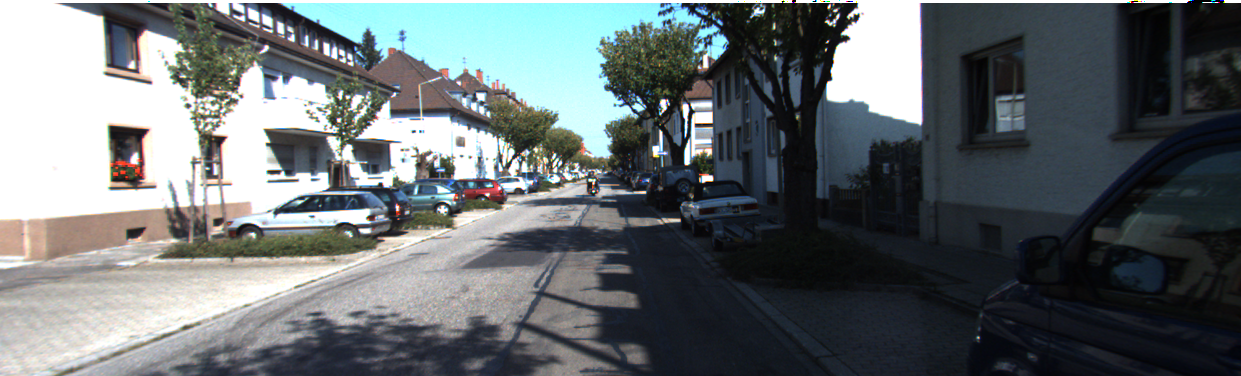
\includegraphics[width=\textwidth]{images/3_1_example_kitti_scene}
    \caption{KITTI - example of scene}\label{fig:example-of-kitti-scene}
\end{figure}

\subsection{Image generation}\label{subsec:kitti-image-generation}
Each sequence of the KITTI dataset is composed of by four sequences of images: left-coloured, right-coloured, left-grey and right-grey.
Each one is captured by a camera mounted on the top of vehicle.
They calibrated the four video cameras intrinsically and extrinsically and rectified the input image.
Then they computed the 3D rigid motion parameters which relate the coordinate system of the laser scanner.

Meanwhile, the ground-truth is directly given by the output of the GPS/IMU localization unit projected into the coordinate system of the left camera after rectification.

\subsection{Dataset statistics}\label{subsec:kitti-dataset-statistics}
The dataset consists of 22 stereo sequences, with a total length of 39.2 km, which was the longest in the time of the publication of the paper.
In the dataset, there are no specifically indicate which sequence is used for training, validation or testing, but in this work, the dataset is split as this:
\begin{table}[H]
    \centering
    \begin{tabular}{|c|c|c|}
        \hline
        \textbf{Sets}           & \textbf{N. of Sequence} & \textbf{N. Image} \\ \hline
        \textbf{Training set}   & 8                       & 20.098            \\ \hline
        \textbf{Validation set} & 2                       & 1.902             \\ \hline
        \textbf{Test set}       & 1                       & 1.201             \\ \hline
        \textit{\textbf{Total}} & 11                      & 23.201            \\ \hline
    \end{tabular}\caption{KITTI - dataset statistics}\label{tab:kitti-dataset-statistics}
\end{table}

The images dimensions about 1240x370 are slightly different, generally varying for few pixels.
\subsection{Usage}\label{subsec:kitti-usage}

This dataset is the one mainly used, as it is the one of the most famous and most used in the literature.

The sequence \textbf{3} and \textbf{7} are used for evaluation and testing, because they are the easier ones.
\begin{figure}[H]
    \centering
    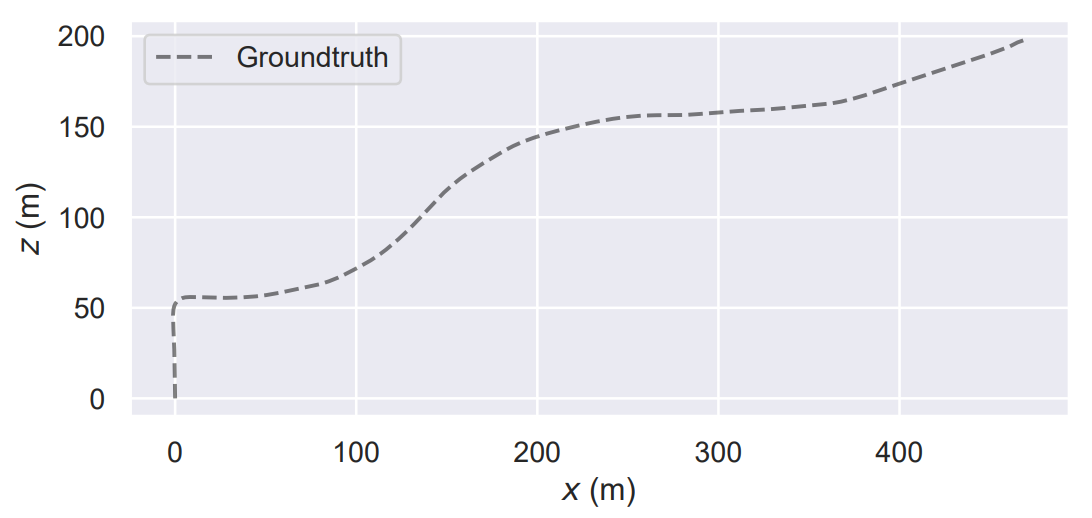
\includegraphics[width=0.5\textwidth]{images/3_1_kitti_seq_3}
    \caption{KITTI - sequence 3}\label{fig:kitti-seq-3}
\end{figure}
\begin{figure}[H]
    \centering
    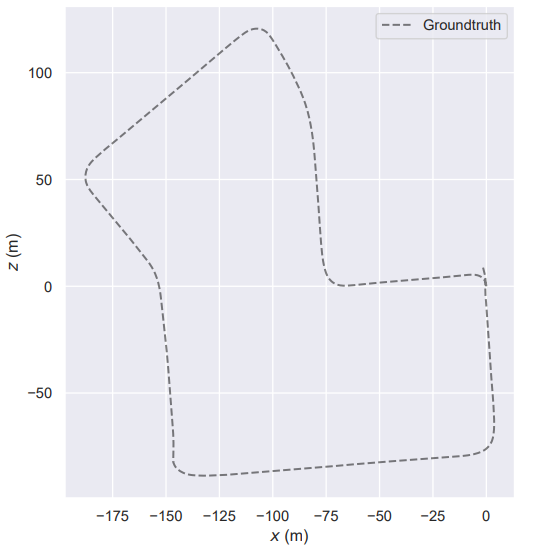
\includegraphics[width=0.5\textwidth]{images/3_1_kitti_seq_7}
    \caption{KITTI - sequence 7}\label{fig:kitti-seq-7}
\end{figure}

Initially, to test the model's capacity, the model was trained and evaluated on the same sequence, to see if it's able to reproduce the ground truth.
Then, the model was fed with more complex sequences.
%
%%**************************************************************
%
% !TEX encoding = UTF-8
% !TEX TS-program = pdflatex
% !TEX root = ./tesi.tex

%**************************************************************
\section{Synthetic}\label{sec:synthetic}
%**************************************************************

As there are few real-life datasets for visual odometry, we decided to create a synthetic dataset by using BlenderProc2 framework,
which is a procedural photo-realistic rendering framework, and it allows to:
\begin{itemize}
    \item \textbf{Loading}: *\textit{.obj}, *\textit{.ply}, *\textit{.blend}, \textit{BOP}, \textit{ShapeNet} etc.
    \item \textbf{Objects}: set or sample objects poses, apply physics and collision checking.
    \item \textbf{Materials}: set or sample physically-based materials and textures.
    \item \textbf{Lighting}: set or sample lights, automatic lighting of 3D-front scenes.
    \item \textbf{Cameras}: set, sample or load camera poses from file.
    \item \textbf{Rendering}: RGB, stereo, depth, normal and segmentation images/sequences.
    \item \textbf{Writing}: *.hdf5 containers, \textit{COCO} and \textit{BOP} annotations.
\end{itemize}

\subsection{Scene}\label{subsec:scene}
To create the synthetic dataset, the first thing is to create a scene with customized objects, material and textures.
\begin{figure}[H]
    \centering
    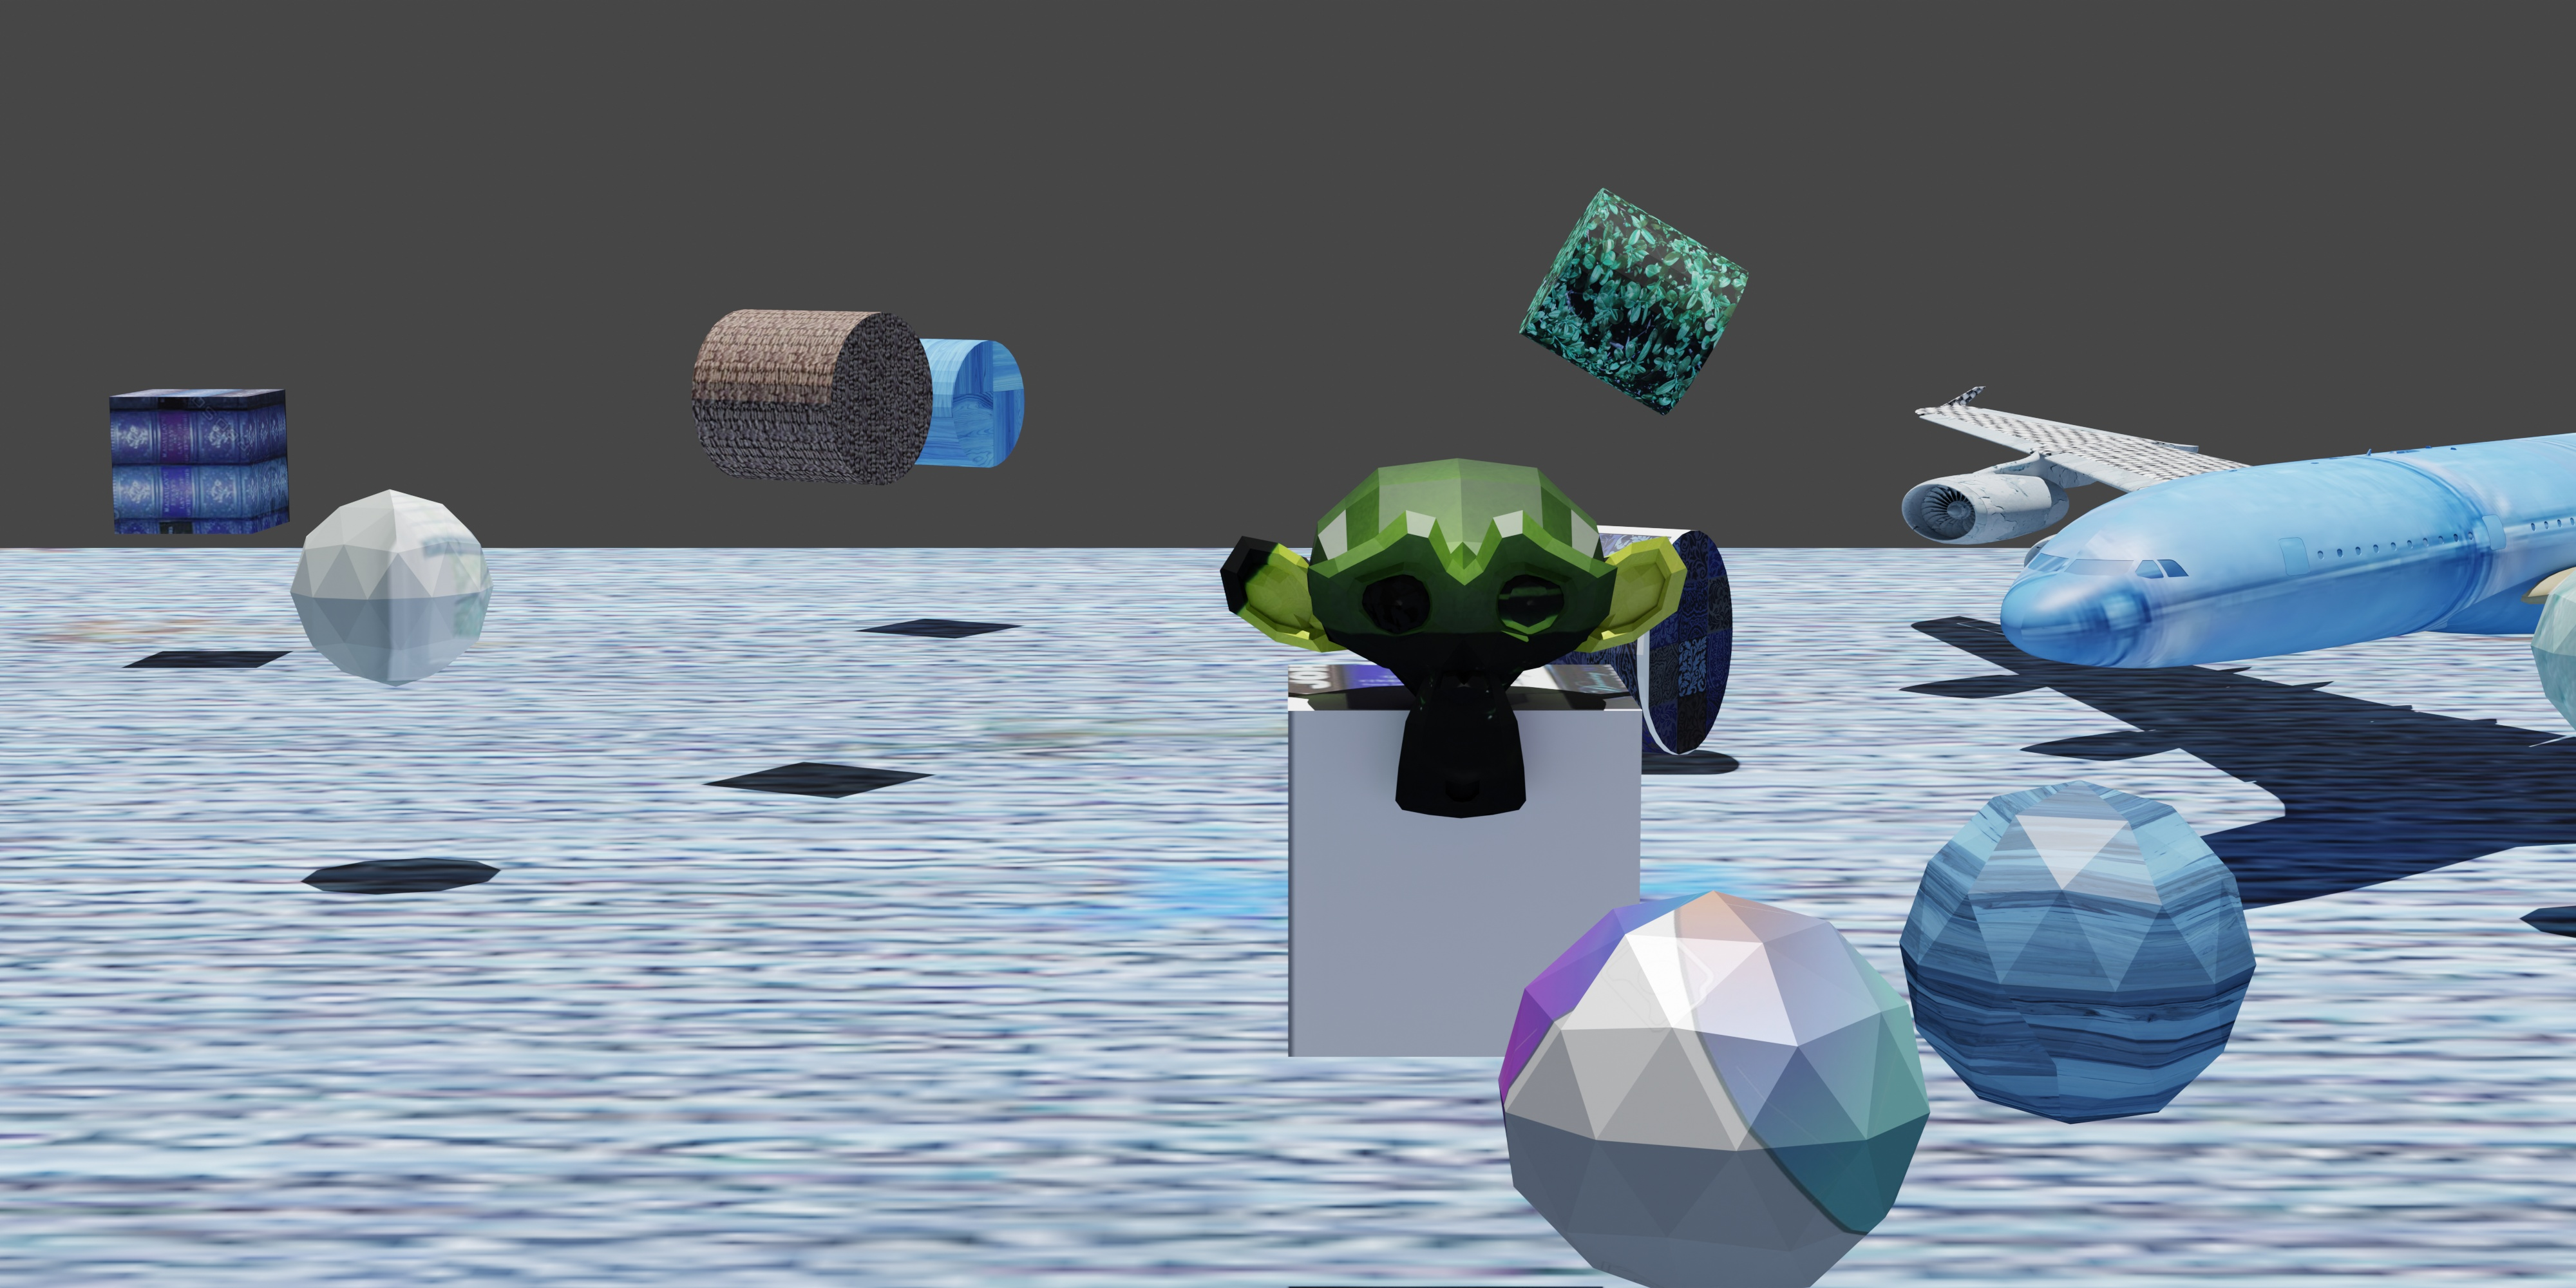
\includegraphics[width=\textwidth]{images/3_example_of_scene}
    \caption{Example of scene}\label{fig:example-of-scene}
\end{figure}
The scene is composed by a set of objects, more precisely:
\begin{itemize}
    \item \textbf{a monkey}: which is at the centre of the scene over a cube.
    \item \textbf{a plane}: which is at left corner of the scene.
    \item \textbf{a set of cubes and spheres}: which are placed randomly in the scene.
\end{itemize}

When rendering the scene, the textures are loaded \textit{randomly}, in the way that in different sequences the textures are different.
\subsection{Image generation}\label{subsec:image-generation}
To generate the sequences, we need to choose the camera position in the scene to do so, we choose randomly a position sampler from the following set for each new pose:

\begin{itemize}
    \item \textbf{disk}: samples a point on a circle or on a 2-ball or on an arc/sector with an inner angle less or equal to 180 degrees.
    \item \textbf{sphere}: samples a point from the surface or from the interior of a solid sphere.
    \item \textbf{part-sphere}: samples a point from the surface or from the interior of a solid sphere which is split in two parts.
    \item \textbf{shell}: samples a point from the volume between two spheres (with radius of the spheres given as parameters).
\end{itemize}
once we have the next position of the camera, we compute the rotation matrix to be applied to the camera in the way that the camera is always looking at the POI (Point Of Interest) which corresponds to the centre of the scene.
\begin{lstlisting}[captionpos=b, label={lst:compute-camera-rotation}, caption={Computes the rotatition matrix for the camera.}, captionpos=b]
rotation = bproc.camera.rotation_from_forward_vec(poi - new_position)
\end{lstlisting}
Then, we apply the rotation matrix to the camera and we generate the image, and by setting a certain number of frames between two poses, the framework renders a sequence of images with relative intermediate poses.


But sometime, it happens that the new camera pose is too close to an object of the scene, so we set two conditions that need to be satisfied, otherwise the sampled camera pose is skipped.
The first condition checks if there are obstacles in front of the camera which are too far or too close based on the given \textit{proximity\_checks}, while the second evaluates the interestingness or coverage of the scene.
\begin{lstlisting}[captionpos=b, label={lst:lstlisting}, caption={Checks whether the camera pose satisfies the conditions.}, captionpos=b]
def check_pose(c2w_m, special_obj, bvh_tree):
    if not bproc.camera.perform_obstacle_in_view_check(c2w_m, {"min": 5.0}, bvh_tree):
        return False
    if bproc.camera.scene_coverage_score(c2w_m, special_objects=special_obj) < 0.7:
        return False
    return True
\end{lstlisting}


But when the new position is too far away from the old position, the rotation of the camera assumes a wrong value during the transition, because it rotates counter-clockwise instead of clockwise, or vice-versa.
For example: if we sample the camera position from a disk at 0, 90, 180, 270 degrees, the rotations should be as in the figure 3.5:
\begin{figure}[H]
    \centering
    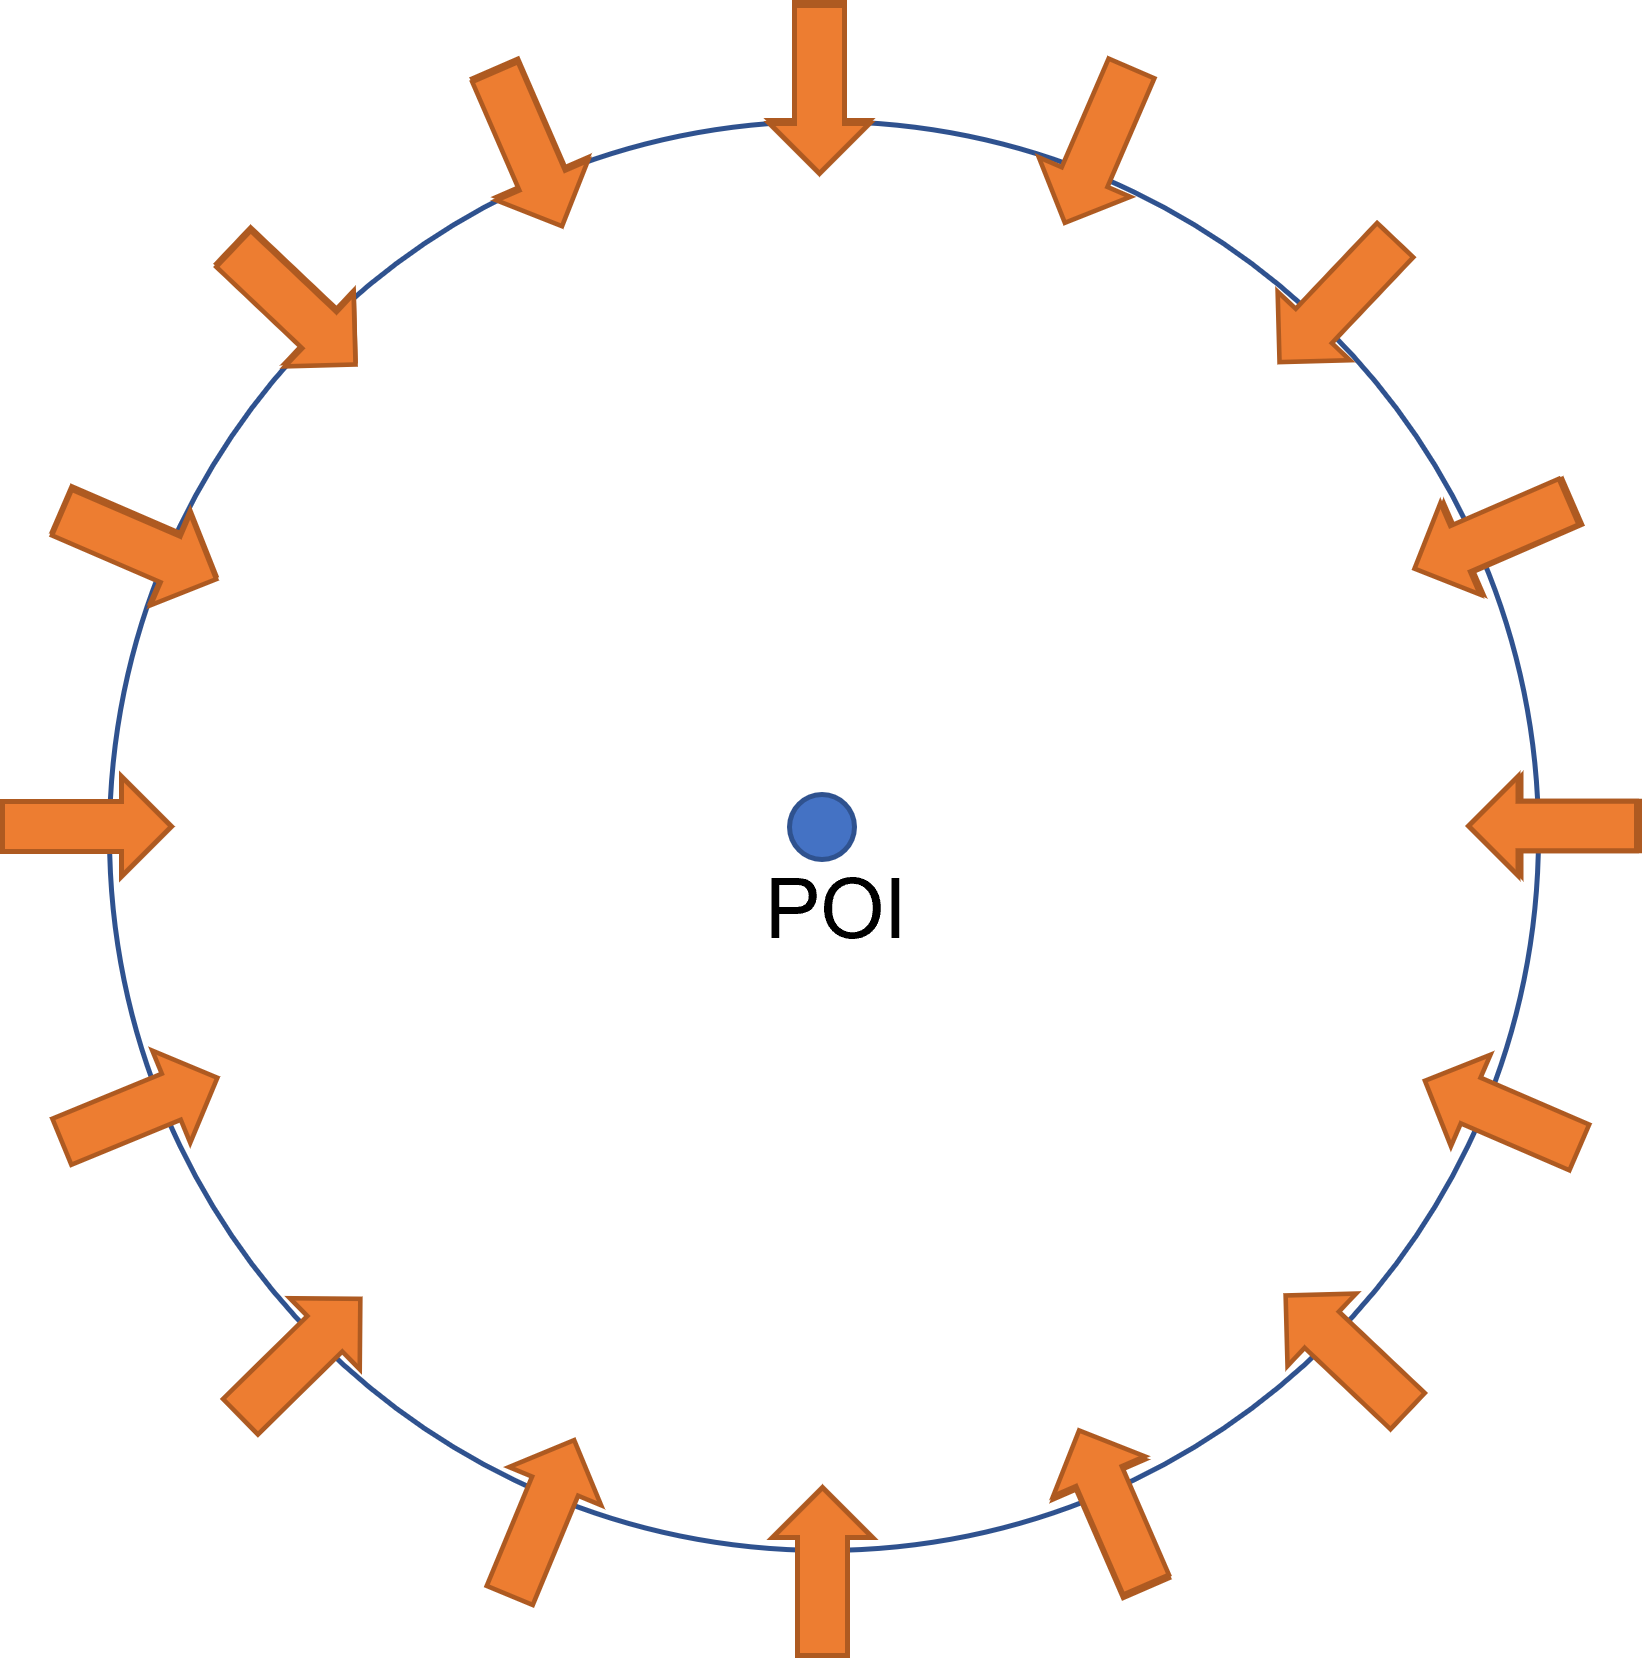
\includegraphics[width=0.5\textwidth]{images/3_correct_transitions}
    \caption{Correct transition on the disk}\label{fig:correct-transition}
\end{figure}

But, the transition from 180 to 270 degrees we obtain is a wrong rotation which is like in figure 3.6:
\begin{figure}[H]
    \centering
    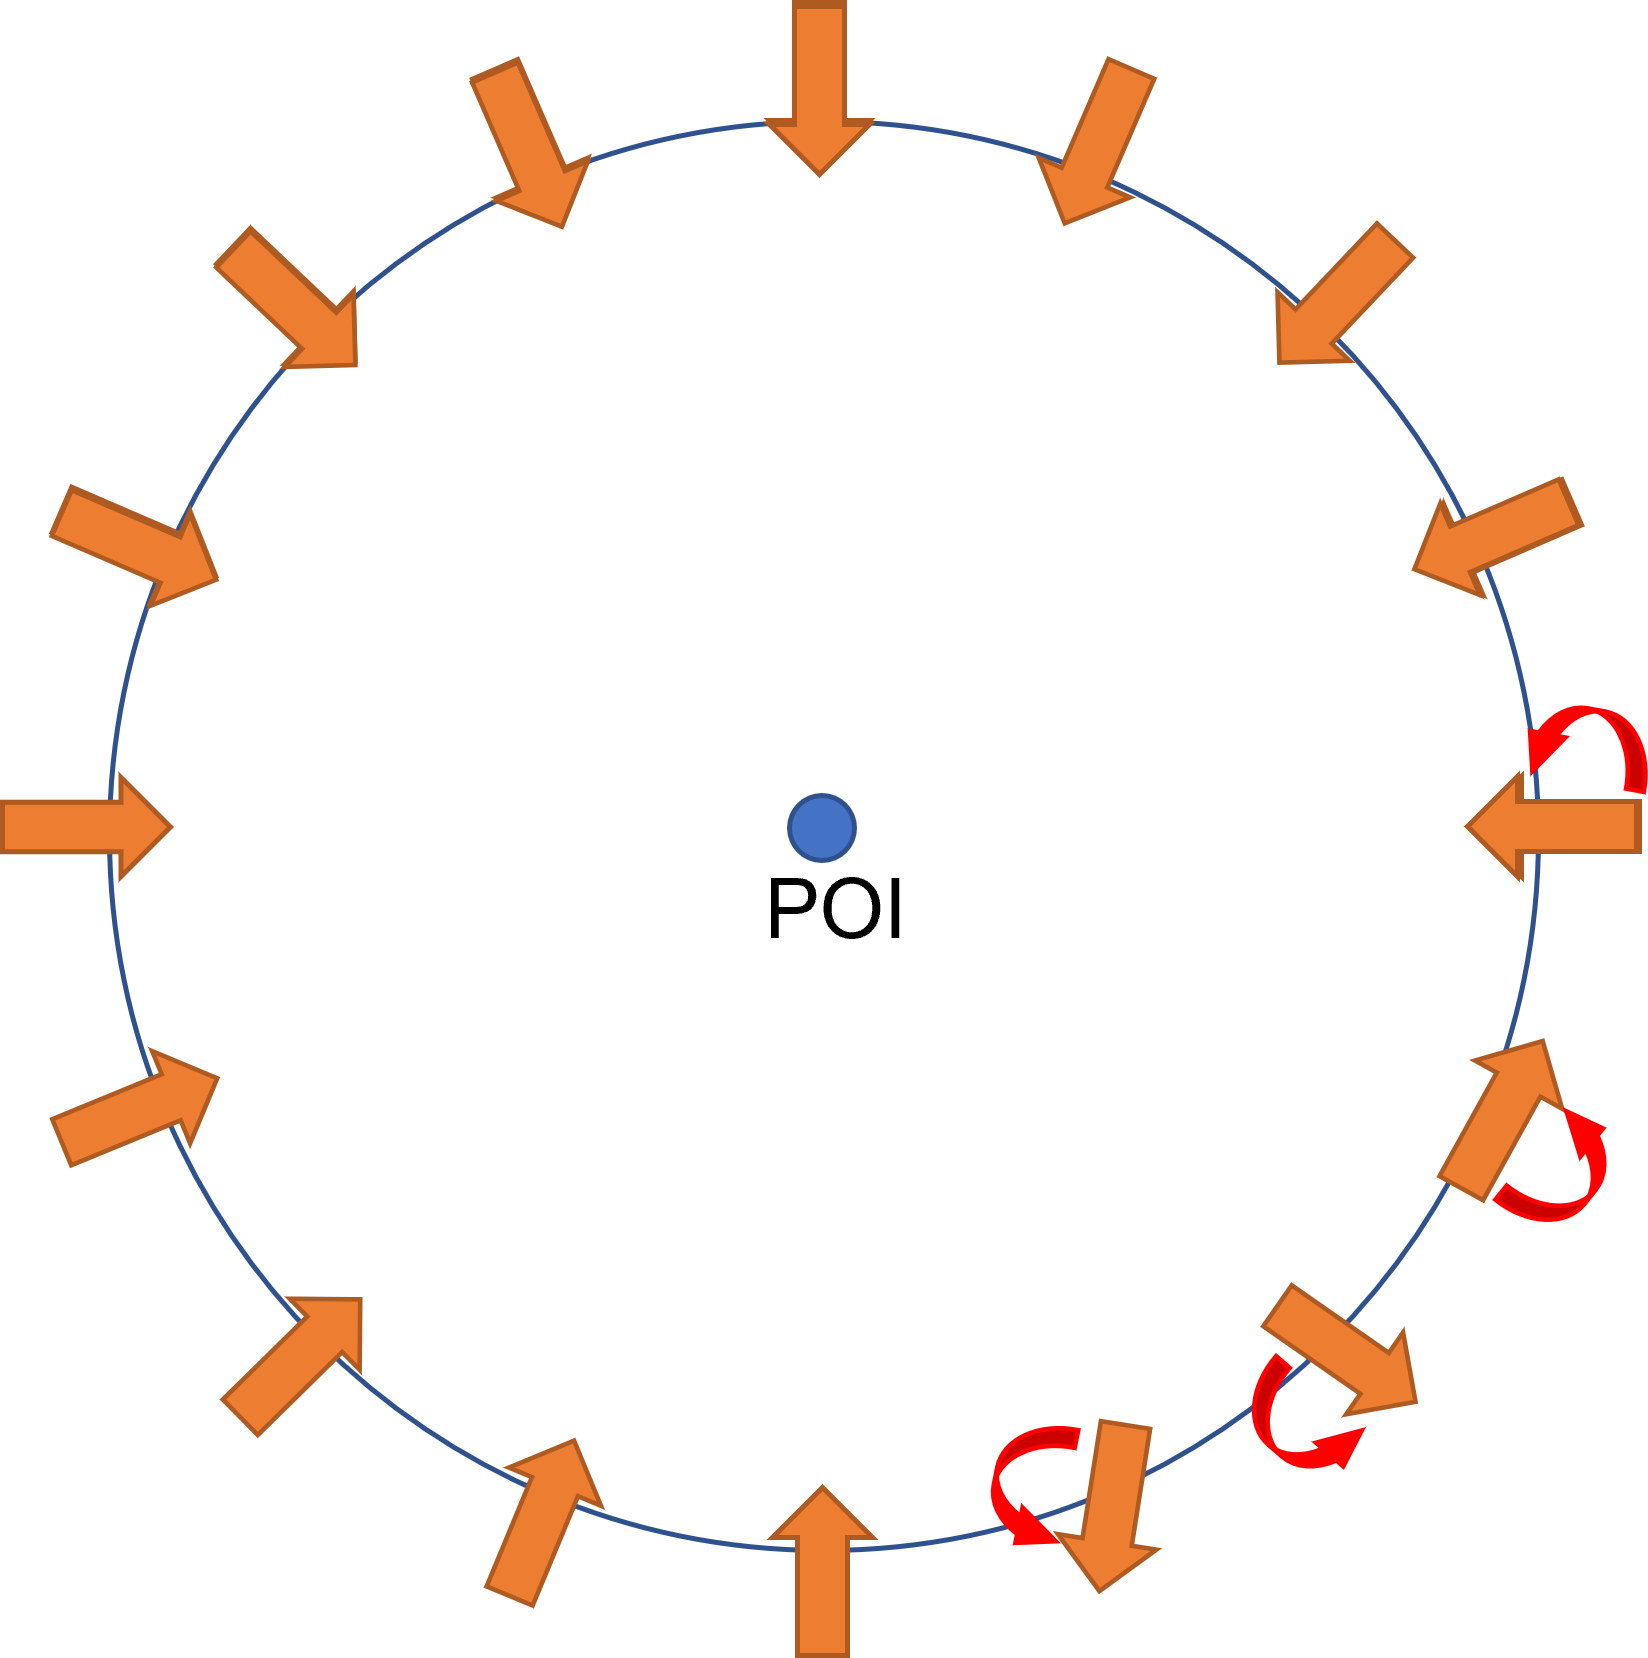
\includegraphics[width=0.5\textwidth]{images/3_wrong_transitions}
    \caption{Wrong transition on the disk}\label{fig:wrong-transition}
\end{figure}

To solve this problem, we tried different solutions: as first, we sample the next pose near to the previous one, but this solution sometime still fails.
The final solution was to sample the new position as previously defined with samplers, but instead of letting the framework to compute the intermediate poses, we manually interpolate them, and by setting frame number to one, we obtain a sequence of correctly rotating images.

\subsection{Dataset statistics}\label{subsec:dataset-statistics}
In total, we have generated 14 sequences, which are divided as follow:
\begin{table}[H]
    \center
    \begin{tabular}{|c|c|c|}
        \hline
        \textbf{Sets}           & \textbf{N. of Sequence} & \textbf{N. Image} \\ \hline
        \textbf{Training set}   & 12                      & 29.100            \\ \hline
        \textbf{Validation set} & 1                       & 1.002             \\ \hline
        \textbf{Test set}       & 1                       & 1.003             \\ \hline
        \textit{\textbf{Total}} & 14                      & 31.105            \\ \hline
    \end{tabular}\caption{Synthetic dataset statistics}
    \label{tab:synthetic-dataset-statistics}
\end{table}
Each image has dimension of 1024x308 pixels with 3 RGB channels.
The whole dateset has dimension \textbf{1.69 GB}.
\subsection{Usage}\label{subsec:usage}
By using the dataset at training time the loss function is highly variable reaching values of \textbf{thousands}, also because the \textbf{Kitti} dataset is much fluid as the trajectory and the camera rotation angles are very small, so, the sequences generated are not similar to the real dataset.
For this reason, we decided to not using this dataset.
%
%%**************************************************************

    % !TEX encoding = UTF-8
% !TEX TS-program = pdflatex
% !TEX root = ../tesi.tex

%**************************************************************


\chapter{Experiments}
\label{ch:experiments}
\intro{In this chapter we will discuss about different models and different prediction strategies.}

%**************************************************************

\section{Models}\label{sec:exp-models}
We designed different models, each one with a different architecture.
These models will be used to test the different prediction strategies.
\subsection{Encoder-only model}\label{subsec:encoder-only-model}
With only-encoder, we mean that the network has only the encoder part, the decoder part is not present.

We tried to use the encoder part of the network to predict the pose of the camera, using both ResNet18 and ResNet50 as feature extractor.
The main difference of ResNet18 and ResNet50 is the number of the output embedding, in fact, ResNet18 has output embedding dimension of 512, while ResNet50 has output embedding dimension of 2048.
We also tried with different depth of the network, depth of \textbf{6} and \textbf{12} layers of encoder.
Then, to obtain prediction, we used a fully connected layer to reduce the dimension of the embedding to the desired number of values, depending on the prediction strategy.
In the figure 4.1 the model architecture is shown.
\begin{figure}[H]
    \centering
    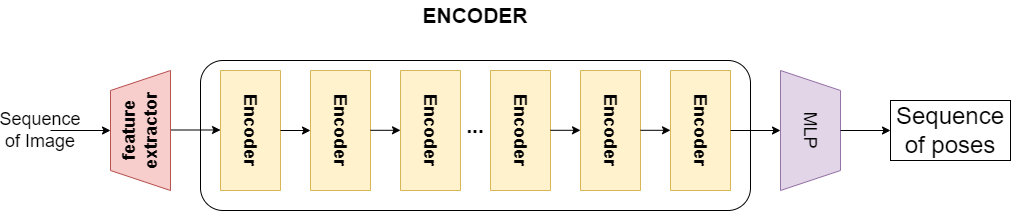
\includegraphics[width=\textwidth]{images/4_1_encoder_only}
    \caption{Encoder-only transformer}\label{fig:figure-encoder-only-transformer}
\end{figure}

\subsection{Encoder-decoder}\label{subsec:encoder-decoder}

For the encoder-decoder, we used the same encoder of the previous section, and we added a decoder part, which takes the output of the encoder as \textit{memory}, and a learnable vector which are also trained.
In this version of the network, we tried the same configurations of the encoder-only model but the feature extractor ResNet50, because the network requires more memory than those available on GPU.
The structure of the network is shown in figure 4.2.
\begin{figure}[H]
    \centering
    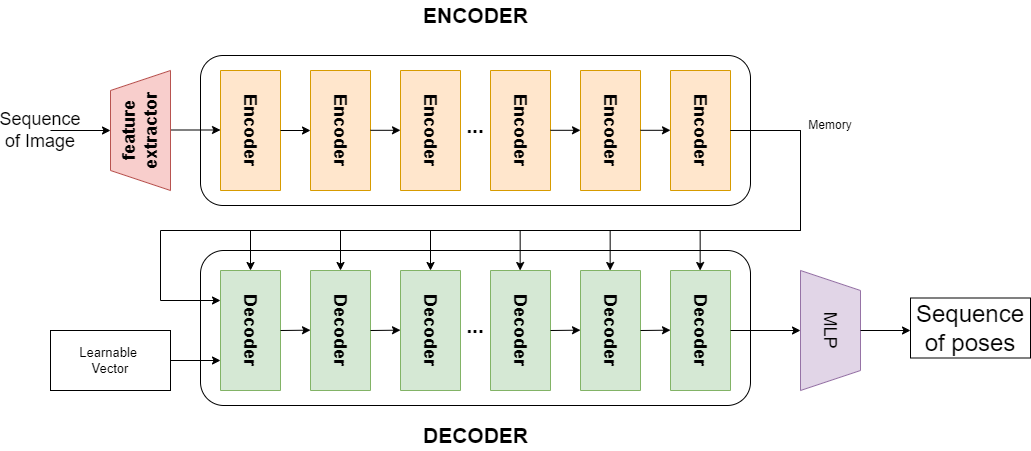
\includegraphics[width=\textwidth]{images/4_1_encoder_decoder}
    \caption{Encoder-Decoder transformer}\label{fig:figure-encoder-decoder-transformer}
\end{figure}

\subsection{Encoder-Decoder with auto-encoder}\label{subsec:encoder-decoder-with-auto-encoder}
In this version of the model, we used the same encoder-decoder model of the previous section, but we added a pose auto-encoder, which given the ground-truth of the pose, it increases the dimensionality of the input to 512 or 2048 and back to the original dimensionality.
The auto-encoder is split into two parts: first part brings the dimensionality from $x$ to 512 and 2048, the second part brings the dimensionality back to $x$, with $x$ depending on the representation format (6 for euler angles, and 12 for roto-translation matrix).
\begin{figure}[H]
    \centering
    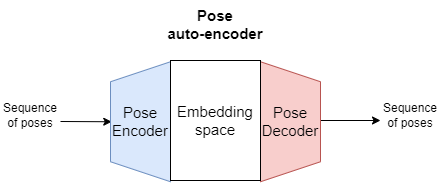
\includegraphics[width=0.5\textwidth]{images/4_1_pose_encoder}
    \caption{Pose auto-encoder}\label{fig:figure-pose-encoder}
\end{figure}

In the Figure 4.3, we can see how the auto-encoder is split in two parts.

We used the first part to create the ground-truth embedding of the pose, the second part to get the prediction of the pose from 512 or 2048 dimensionality.
So, the final structure of the model is shown in Figure 4.4.
\begin{figure}[H]
    \centering
    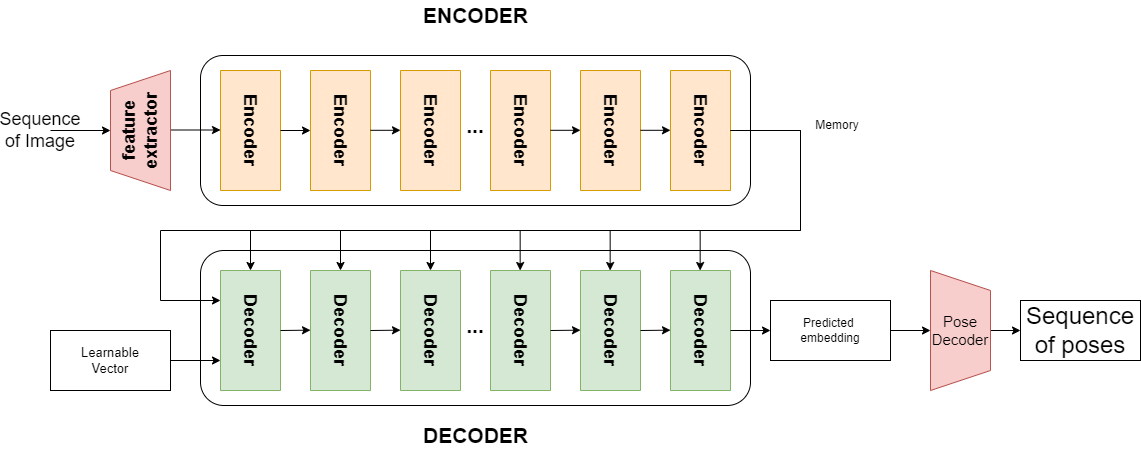
\includegraphics[width=\textwidth]{images/4_1_encoder_decoder_with_pose_autoencoder}
    \caption{Encoder-Decoder with pose auto-encoder}\label{fig:figure-encoder-decoder-with-pose-encoder}
\end{figure}

\subsection{Encoder-Decoder in autoregressive mode}\label{subsec:encoder-decoder-in-autoregressive-mode}
In this model, we replaced the parameter vector \textit{memory} with the output of the first part of the pose auto-encoder because the output is used to generate the ground-truth embedding used as target embedding, and the second part, as usual, is used to calculate the pose from embedding.

\begin{figure}[H]
    \centering
    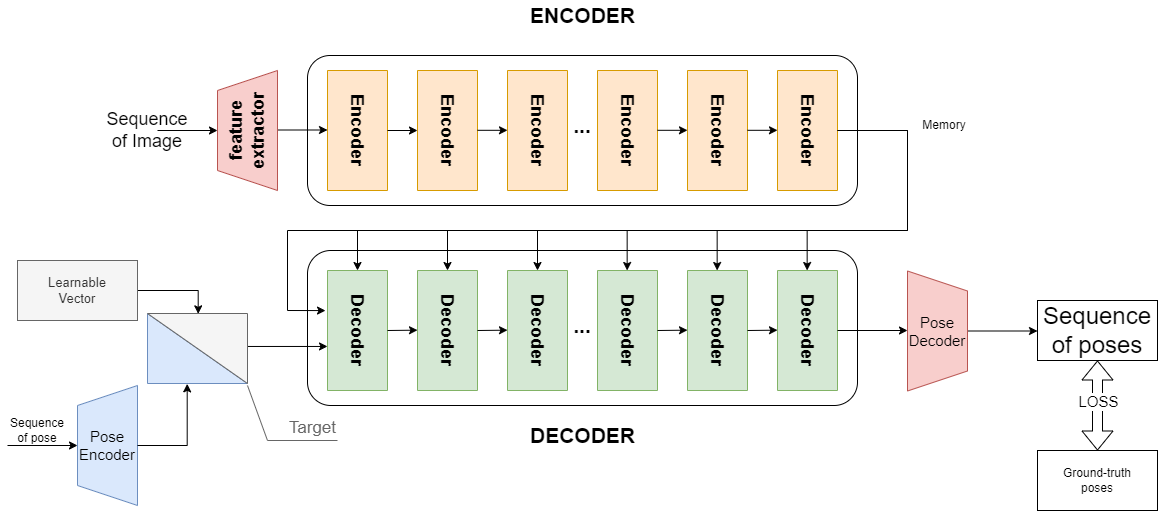
\includegraphics[width=\textwidth]{images/4_1_ar_train}
    \caption{Auto-regressive mode: training time.}\label{fig:figure-auto-regressive-train}
\end{figure}

In the figure 4.5, we can see the architecture of this model at \textbf{training time}, where the memory comes from the encoder, then, we construct the target by using the learnable vector as the upper-triangle of the target, and the embedding of the ground-truth as the lower-triangle of the target.
For the \textbf{inference time}, where we need to predict the pose one by one, starting from the second pose because the first one is the origin, in the figure 4.6, we can see the workflow of the model.
At first step of prediction, where we have to predict the second pose, we use the target which is composed like: $[origin\_emb, learnable\_vector[1\colon-1]]$ , for next step,
we will use: $[origin\_emb, first\_prediction, learnable\_vector[2\colon-1]]$, then $[origin\_emb, first\_prediction, second\_prediction, learnable\_vector[3\colon-1]]$, and so on so forth.
Meanwhile, the memory is not changed.

\begin{figure}[H]
    \centering
    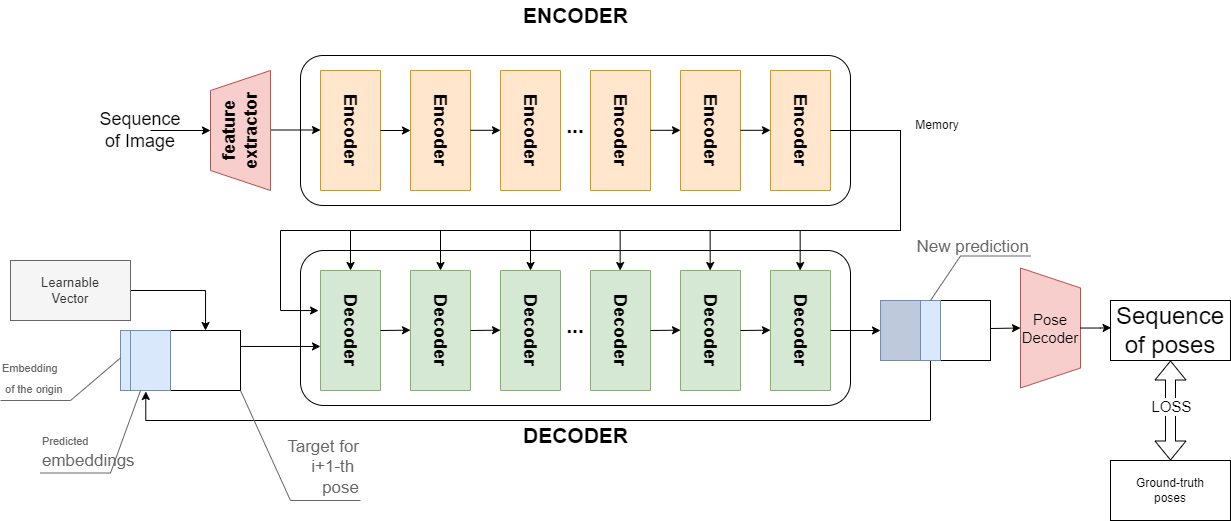
\includegraphics[width=\textwidth]{images/4_1_ar_inference}
    \caption{Autoregressive mode: inference time}\label{fig:figure-auto-regressive-inference}
\end{figure}


%**************************************************************

\section{Feeding Strategies}\label{sec:prediction-strategies}
To solve the problem of visual odometry, we tried different approaches to feed the sequence of image into the model, and to construct the model itself.
We tried following approaches to feed the data:
\begin{enumerate}
    \item Feeding the sequence into the model directly and representing the pose as \emph{euler angles}.
    \item Feeding the sequence into the model directly and representing the pose as \emph{rotation matrix} so with twelve numbers and \emph{translation vector}.
    \item Feeding the sequence into the model where the first frame is the origin of the reference frame and representing the pose as \emph{euler angles}.
    \item Feeding the sequence into the model where the first frame is the origin of the reference frame and representing the pose as \emph{rotation matrix} and \emph{translation vector}.
    \item Feeding the sequence into the model where the first frame is the origin of the reference frame, and using the auto-regressive model to predict the pose.
\end{enumerate}
We can divide these strategies into two groups: the first group is composed by strategy 1 and 2, and the second group is composed by strategy 3, 4 and 5.
This division is because the first group uses the ground-truth without any preprocessing, meanwhile the second group uses the ground-truth translated with respect to the first pose of the sequence.

\subsection{Directly feeding the sequence}\label{subsec:directly-feeding-the-sequence}
With this strategy, we create each sequence by taking the images from the dataset and the pose as ground-truth without any processing.
For the sake of simplicity, to explain the different strategy, we will use an example of trajectory which is as represented in the Figure 4.7:
\begin{figure}[H]
    \centering
    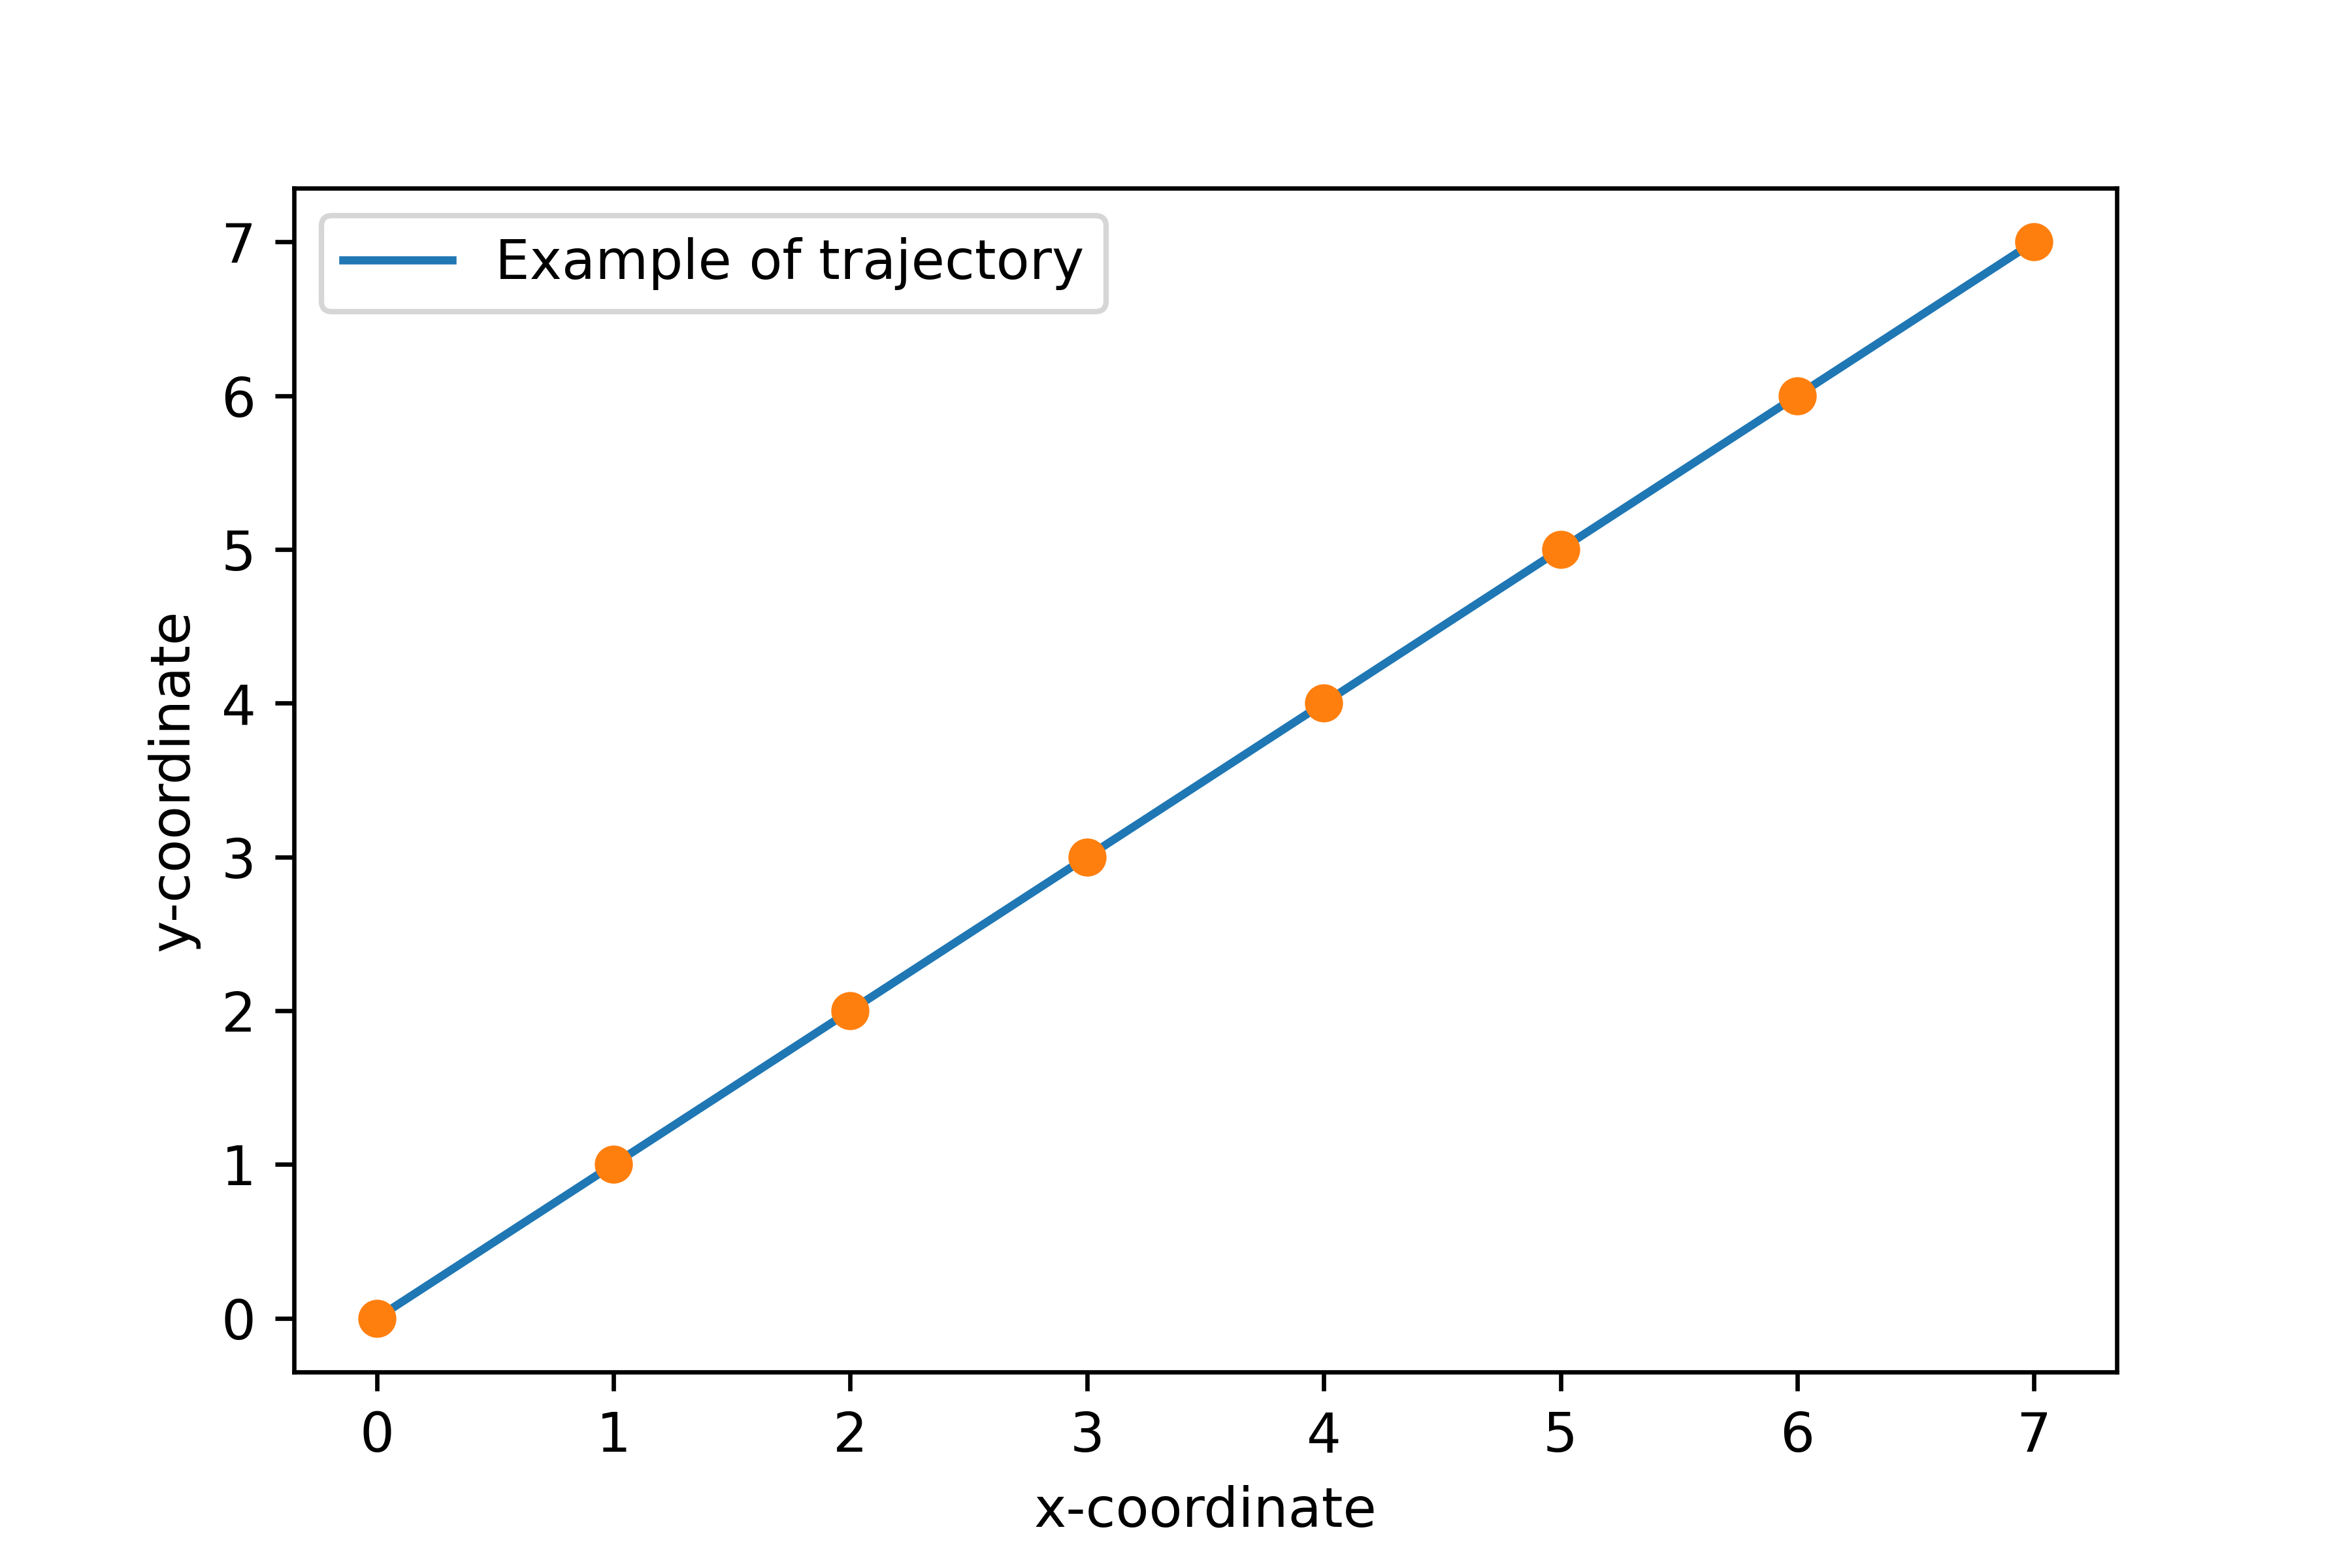
\includegraphics[width=\textwidth]{images/4_2_example_of_trajectory}
    \caption{Example of the trajectory.}
    \label{fig:example-of-trajectory}
\end{figure}
Of course, in the example the trajectory looks easy to predict because the distance between every pair of pose is the same, and trajectory direction is not changing.
Meanwhile, in the KITTI dataset, the trajectories are more complex, and the distance between the poses is not constant, and the direction of the trajectory is changing.
We can see the trajectory where each dot represents an image-pose pair.
From this trajectory, we can represent the dataset and  the creation of the sequences as follows:
\begin{figure}[H]
    \centering
    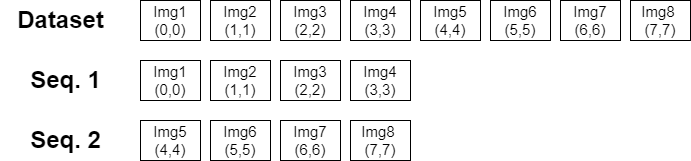
\includegraphics[width=\textwidth]{images/4_2_directly_feeding}
    \caption{Example of the dataset and the sequences.}
    \label{fig:example-of-dataset}
\end{figure}
This way of feeding the data is the simplest one, but it has some drawbacks.
The first one is that when we split the training dataset into different sequences, for each sequence, the coordinates do not start from the origin (i.e., (0,0)) but for example for the second sequence, it starts from (4,4).
This is problematic for the model because it has to learn this kind of translation, and it is not a trivial task.
The second drawback is that the model has to predict a very large interval of numbers in this case, the range goes from 0 to 7, but in real case, like in the KITTI dataset, the range goes from 0 to 1000.
The third drawback is that, with a dataset of $N$ images, we can have only $\frac{N}{seq\_len}$ sequences, where $seq\_len$ is the length of the sequence, this aggravates on the problem of small dataset available.


\subsection{Sequence with origin}\label{subsec:sequence-with-origin}
In this second strategy, we create each sequence by taking the images from the dataset, and the pose as ground-truth by performing a translation operation.
In this way, the sequences can be represented as follows:
\begin{figure}[H]
    \centering
    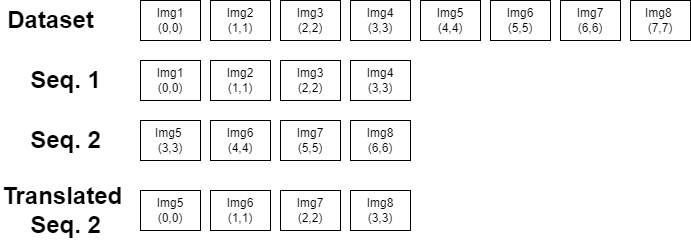
\includegraphics[width=\textwidth]{images/4_2_split_traj_1}
    \caption{Example of the dataset with origin and the split of sequences.}
    \label{fig:example-of-dataset-with-origin}
\end{figure}
We can see that the sequences start from the origin, and the model has to learn only the relative pose to the first frame of the sequence, instead of the whole trajectory.
But this solution is not perfect, in the sense that, in this trajectory we have eight image-pose pair, and with $seq_len = 4$ we can generate only two sequences, and considering that the Kitti dataset has about 20.000 images, this is a big problem.

To solve the previous mentioned problem, we devised a slightly modified strategy, which essentially takes every image-pose pair and creates a sequence of length $seq\_len$, like represented in Figure 4.10:
\begin{figure}[H]
    \centering
    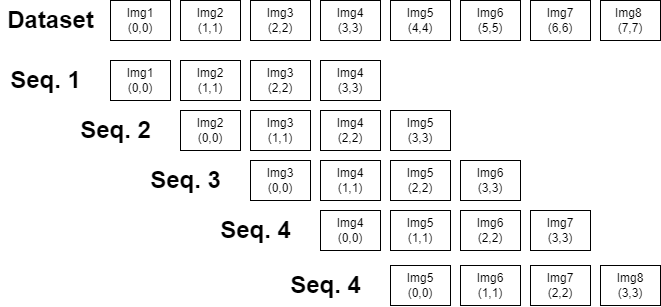
\includegraphics[width=\textwidth]{images/4_2_split_traj_2}
    \caption{Example of the dataset with origin.}
    \label{fig:example-of-dataset-with-origin-2}
\end{figure}
As represented in the previous figure, with a dataset of $N$ images, we can have $N - seq\_len +1 $ sequences, and this is a big improvement with respect to the previous strategy.
Also, in this way, we are doing a sort of data augmentation, because we're feeding the model with different sequences, and this is helpful for the model.

As comparison, with first strategy, using KITTI dataset, we can have only $\frac{N}{seq\_len}$ sequences, where $N = 20.000$ and $seq\_len = 4$, so we can have only $5000$ sequences, while with the latest strategy, we can have $N - seq\_len +1$ sequences, so we can have $19997$ sequences, which is an important improvement.


%**************************************************************

    % !TEX encoding = UTF-8
% !TEX TS-program = pdflatex
% !TEX root = ../tesi.tex

%**************************************************************


\chapter{Implementations}\label{ch:implementations}
\intro{In this chapter we will discuss about the implementations of different components of the project and the reason that led us to such choices.}

%**************************************************************

\section{Dataset preprocessing}\label{sec:dataset-preprocessing}

Before feeding the sequence of images into the model, as it is usual in the literature, we need to preprocess the images.

The first operation is the normalization (dividing each pixel value by 255) in order to have the images in the range $[0,1]$, this is useful because the neural network works better with this range as it has to compute smaller range of numbers.
The second operation is the standardization, in this way, we are centering the data around zero, and we are reducing the variance of the data, to do so, we computed the mean for each of RGB channels following this formula:
\begin{equation}
    \mu_{c} = \frac{1}{HW}\sum_{i=1}^{H}\sum_{j=1}^{W}I_{c}(i, j)
    \label{eq:equation_mean}
\end{equation}
where $I_{c}(i, j)$ is the $j$-th pixel of the $i$-th row of the $c$-th channel, $W$ is the width of the image, $H$ is height of the image, $\mu_{c}$ is the mean of the $c$-th channel.
Then, the standard deviation as follow:
\begin{equation}
    \sigma_{c} = \sqrt{\frac{1}{HW}\sum_{i=1}^{H}\sum_{j=1}^{W} (I_{c}(i,j) - \mu_{c})^{2}}
    \label{eq:equation_std_dev}
\end{equation}
where $\sigma_{c}$ is the standard deviation of the $c$-th channel.
Finally, we normalized the images as follow:
\begin{equation}
    I^*_{c}(i) = \frac{I_{c}(i,j) - \mu_{c}}{\sigma_{c}}
    \label{eq:equation_normalization}
\end{equation}
$\forall i \in [1, H], j \in [1, W], c \in [R, G, B]$ and $I^*_{c}(i)$ is the normalized $i$-th pixel of the $c$-th channel.

We perform the aforementioned operations to all images of the KITTI dataset saving new images, in this way, we need to process them just once, saving time during the training process.



%**************************************************************

\section{Data Loading}\label{sec:data-loading}
The data-loading process is strictly connected to the \hyperref[]{\S4.2 Experiments - Feeding strategies}, because it changes how we want to feed the data to the neural network.

This process is divided into two parts, the first one is the loading process, and the second one is how to draw a batch of sequences.

\subsection{Loading process}\label{subsec:loading-process}
Initially, we load the images and the poses into the RAM from the KITTI dataset, so in the same time we require the computer to keep in memory a lot of images.
And, this is not efficient from a point of view of memory.

Then, we decided to store only the path to the images and the poses in the RAM, and we load the images and the poses from the disk when we need them.
This is a good solution because we don't need to keep in memory all the images, but we need to load them from the disk when we need them.
So the performance of the disk where we store the images is important.

To perform this, we created a class called \textit{KittiDataset} that inherits from the \textit{Dataset} class of the \textit{PyTorch} library.
And, by overriding the \textit{\_\_getitem\_\_} and \textit{\_\_len\_\_} method, we can load the images and the poses from the disk when we need them.

Then, the last operation we do is to resize the images to (1200, 360), this is to ensure that all the images has the same size.

\subsection{Batch drawing}\label{subsec:batch-drawing}

The batch drawing is the process of drawing a batch of items from the dataset.
In our case, each item is a sequence of images and poses.

The API pytorch provides for this is the \textit{DataLoader} class, which takes in input a dataset object.
By default, the Dataloader class shuffles the dataset, and it draws a batch of items from the dataset, it processes them with \textit{collate\_fn} function, and it returns them.

The \textit{collate\_fn} function is a function that takes in input a list of items, and it returns a tuple of tensors.
The first one is the input for the NN, so the images, and the second one is the target, so the poses.

Another important parameter of the class \textit{DataLoader} is Sampler or BatchSampler.
The difference between them is that with Sampler we can customize how to select items from the dataset, influencing the choice of the dataloader over items, meanwhile, the BatchSampler is used to customize how to select batches from the dataset, influencing the choice of the dataloader over one batch.

To implement the first strategy of \hyperref[]{\S4.2.2 Experiments - Feeding strategies} we implemented a BatchSampler that draws a batch of sequences, such that each item (sequence) is connected to the one before and after it.

But, for the final version (Second one introduced in \S4.2.2), we use the default sampler, because we implemented the dataset \textit{\_\_getitem\_\_} method in a way that it returns a sequence of images and poses.
E.g., when the $item_i$ is requested, the method returns a sequence from $item_i$ to $item_{i + seq_{len}-1}$.
The \textit{\_\_getitem\_\_} method also processes the poses in a way the pose of the first image is the origin of the coordinate system and the origin of the sequence.
\begin{lstlisting}[captionpos=b, language=python,label={lst:dataset-get-item}, caption ={The \textit{\_\_getitem\_\_} method of the \textit{KittiDataset} class.}]
def __getitem__(self, idx):
    images, poses  = [], []
    to_translation, to_rotation = None, None
    for i in range(idx, idx + self.seq_len):
        img_path, pose = self.data[i]
        rot, tran = pose[:3, :3], pose[:, -1]
        if to_translation is None:
            to_translation, to_rotation = tran, rot
        tran = tran - to_translation
        rot = rot @ torch.t(to_rotation)
        pose = torch.cat((rot, tran.reshape(3, 1)), dim=1).reshape(-1, )
        frame = load_image(img_path, self.transform)
        images.append(frame)
        paths.append(img_path)
    return images, poses
\end{lstlisting}
In this way, we can randomly sample sequences from the dataset, removing the constraint of the connection between the sequences.

When we train the network, we set the shuffle parameter to \textbf{True}, to \textbf{False} during th test time, because we want to have the sequences in the same order as in the dataset to be able to reconstruct the trajectory.
To reconstruct the trajectory, we need to obtain the prediction of each sequence, then re-concatenate them as \text{Code. 5.2} shows:
\begin{lstlisting}[captionpos=b, language=python,label={lst:reconstruct-trajectory}, caption ={Reconstruct the trajectory from the predictions which is a list of batches of sequences.}]
def composing_trajectory(predictions):
    trajectory = []
    back_translation = predictions[0, 0, 0].reshape(3, 4)[:3, -1]
    back_rotation = predictions[0, 0, 0].reshape(3, 4)[:3, :3]
    trajectory.append(torch.cat((back_rotation.reshape(3, 3), back_translation.reshape(3, 1)), dim=1).flatten())
    for k in range(predictions.shape[0]):
        # number of batches
        for i in range(predictions.shape[1]):
            # number of sequence in each batch
            for j in range(predictions.shape[2]):
                # number of frames in each sequence
                current_pose = predictions[k, i, j].reshape(3, 4)
                rot, tran = current_pose[:3, :3], current_pose[:3, -1]
                if j == 0: # beginning of the sequence
                    last_pose = trajectory[-1].reshape(3, 4)
                    back_translation = last_pose[:3, -1]
                    back_rotation = last_pose[3, :3]
                else:
                    tran = tran + back_translation
                    rot = rot @ back_rotation
                    trajectory.append(torch.cat((rot.reshape(3, 3), tran.reshape(3, 1)), dim=1).flatten())

    return torch.stack(trajectory)
\end{lstlisting}
Where the \textit{predictions} is a tensor of shape \textit{(num\_batchs, batch\_size, seq\_len, 12)}, i.e., a list of batches.


%**************************************************************
\section{Models}\label{sec:models}
%**************************************************************

\subsection{Standard model}\label{subsec:standard-model}
We used PyTorch deep-learning framework to implement the models because it's flexible, intuitive, and easy to use.
We mainly used ResNet18 and ResNet50 as \textbf{feature extractor}, we used the pre-trained version of these models, which are trained on ImageNet dataset by the authors of the library.

We took the model, removed the last layer, in this way, as output of the layer we obtain a tensor of size 512 or 2048, depending on the model, and we used this as the embedding.

Then, we used the \textit{TransformerEncoderLayer}, \textit{TransformerEncoder}, \textit{TransformerDecoderLayer}, and \textit{TransformerDecoder} from the PyTorch library.
Where TransformerEncoder is single layer, TransformerEncoderLayer is the container for the encoder layers, and it takes as input the number of layers.
Meanwhile, the TransformerEncoder needs as input:
\begin{itemize}
    \item \textit{embedding dimension}: 512 or 2048, depending on the feature extractor;
    \item \textit{n\_head}: the number of attention heads;
    \item \textit{mlp\_dim}: the number of neurons in the MLP;
    \item \textit{drop\_out}: the dropout rate;
\end{itemize}
The output of the Encoder is known as memory.
The TransformerDecoder and TransformerDecoderLayer are similar to the TransformerEncoder and TransformerEncoderLayer, respectively.
The difference between TransformerEncoderLayer and the TransformerDecoderLayer is that the latter in \textit{forward} method, it takes as mandatory parameter the target sequence, while the former doesn't.
There are also some optional parameter, like the \textit{src\_key\_padding\_mask} and \textit{src\_key\_padding\_mask}, which functionality is explained in \hyperref[subsec:transformer]{\S2.1.2 Theoretical foundations - Transformer}.

Finally, depending on different version of the model we introduced in \hyperref[subsec:models]{\S4.1 Experiments - Models}, we used different MLP to predict the pose.

\subsection{Auto-regressive model}\label{subsec:auto-regressive-model}
What we want to do is to predict the future poses of the sequence, given the past poses.
In details, we want to predict the pose at time $t_i$, given the poses at time $t_0, t_1, \dots, t_{-i-1}$.
To do this, we should treat the training time and the inference time differently.

In the training phase, we feed the decoder with the memory and the target, which is obtained by combining the ground-truth pose embedding, and the learnable vector (with the same shape of a sequence), the combination is defined as follows:
\begin{lstlisting}[captionpos=b, label={lst:lst-training-target}, caption={Training target}, language=Python]
def _training_target(self, gt):
    """
    :return: the target for the training phase, that should be:
    [
    [GT, trg, trg, trg, trg],
    [GT, GT,  trg, trg, trg],
    [Gt, GT,  GT,  trg,  trg],
    [Gt, GT,  GT,  GT,  trg]
    ]
    """
    learnable_target = repeat(self.learnable_target, 'n d -> b n d', b=gt.shape[0])
    lower_triangular = torch.tril(gt)
    upper_triangular = torch.triu(learnable_target, 1)
    return lower_triangular + upper_triangular
\end{lstlisting}
In the example, from code snippet 5.3, each row is a sequence of poses, and each element of the row is a pose.
\textit{GT} is the ground-truth pose embedding computed by the pose auto-encoder, meanwhile the \textit{trg} is part of the learnable vector.
In the example, the batch\_size is 4 and seq\_len is 5.
With this target, at the time 0, we have the \textit{GT} at first pose, also because it's considered the origin of that sequence, then what we have to predict is the second pose.
For the second sequence, we have \textit{GT} at pose 0 and 1, and we have to predict the pose 2.
And so on so forth.
Last thing we should pay attention to is that the loss should be computed only for the elements on the first diagonal of the matrix, because in the lower triangular matrix, we have the ground truth, and we don't care about the predictions of the upper triangular matrix.

At inference time, the target for the decoder is composed by it-self's output at previous time step combined with the learnable vector as the following function:
\begin{lstlisting}[captionpos=b, label={lst:lst-inference-target}, caption={Inference target}, language=Python]
def _inference_target(self, predictions, column_index):
    """
    column_index is the index of the column that we want to predict: always 0 < x < seq_len
    :return: the target for the inference phase, that should be:
    for column_index = 1:
    [
    [GT, trg, trg, trg, trg],
    ...
    [GT, trg, trg, trg, trg],
    ]
    for column_index = 2:
    [
    [GT, GT, trg, trg, trg],
    ...
    [GT, GT, trg, trg, trg],
    ]
    """
    # origin_embed shape: batch_size, 1, emb_size,
    # learnable_target shape: batch_size, seq_len, emb_size
    # predictions shape: batch_size, seq_len, emb_size
    return torch.cat((predictions[:column_index, :], self.learnable_target[column_index:, :]), dim=0)
\end{lstlisting}

The code for inference is the following the one shown in \textbf{Code 5.5}.
\begin{lstlisting}[captionpos=b, label={lst:lst-inference}, caption={Inference}, language=Python]
predictions = torch.zeros_like(x)
predictions[:, 0, :] = gt_target  # embedding of the origin
for i in range(1, x.shape[0]):
    new_target = self._inference_target(predictions[i], i).unsqueeze(0)
    predicted = self.decoder(new_target, x[i].unsqueeze(0), tgt_mask=generate_upper_triangular_mask(x.shape).to(self.device))
    predictions[i, :, :] = predicted[:, :, :]
    if i < x.shape[0] - 1:
        predictions[i + 1, :, :] = predicted[:, :, :]
\end{lstlisting}
In the previous code snippet, the \textit{gt\_target} origin embedding, we instantiate a tensor with the same shape of the input, we set the first column to the origin embedding, and then we iterate over the sequence.
At each iteration, we predict the pose at $i$-th, given the previously predicted poses at time $t_0, t_1, \dots, t_{i-1}$ for all the sequences of the batch.
Differently from the training, we should compute the loss for the whole \textit{predicted} tensor, because we are predicting all the poses.


%**************************************************************
\section{Losses}\label{sec:losses}
Loss function is an important component of the training process, it is used to evaluate the performance of the model, and by optimizing it (minimizing it or maximizing it) we can improve the performance of the model.
In our case, we tried different loss functions:
\begin{itemize}
    \item Mean Squared Error (MSE);
    \item Weighted MSE;
\end{itemize}

\subsection[Mean Square Error]{Mean Square Error (MSE)}\label{subsec:mean-square-error-(mse)}
MSE is the most common loss function used in regression problems.
Given the ground truth pose $p_{gt}$ and the predicted pose $p_{pred}$, the MSE is defined as:
\begin{equation}
    \label{eq:mean-square-error}
    MSE = \frac{1}{N} \sum_{i=1}^{N} (pose_{gt} - pose_{pred})^2
\end{equation}

This loss function is derived from the square of Euclidean distance, it is always positive value that decreases as the error approaches zero.

\subsection[Weighted Mean Square Error]{Weighted Mean Square Error-WMSE}\label{subsec:weighted-mean-square-error-wmse}
WMSE is a variation of the MSE, which is useful when we want to give more importance to some components of the pose.
For example, given a sequence of poses: $p_0$, $p_1$ \dots $p_n$, we want to give more importance to the poses more distant from the origin, because we want the poses far away from the origin to be closer to the ground truth.
In this way, we impose the network to give more importance for the poses far away from the origin as the errors accumulate over steps.
The formula of the WMSE is:
\begin{equation}
    \label{eq:weighted-mean-square-error}
    WMSE = \frac{1}{N} \sum_{i=1}^{N} i * (pose_{gt} - pose_{pred})^2
\end{equation}
In the equation, we chose $i$ as the weight of the pose, but we can use any other function of $i$.


%**************************************************************

\section{Pose auto-encoder}\label{sec:pose-auto-encoder}
Pose encoder structure is very simple, it takes as input the pose, and it outputs the same pose.
We devised this a MLP can be get in input the pose, and it can reproduce the same poses with small margin of error.
In fact, we discovered that with \hyperref[subsec:directly-feeding-the-sequence]{\S4.2.1 Experiments - Feeding strategies}, the auto-encoder really struggles to reduce the loss, MSE in this case, the reason is that the network is required to output a very large range of values.
To fix this, we are forced to used \hyperref[subsec:sequence-with-origin]{\S4.2.2 Experiments - Feeding strategies}.
Another reason is that by use ReLU activation function, the network is forced to output only positive values, meanwhile for some poses, the output of the network is negative.
To solve this problem, we used LeakyReLU activation function, which allows the network to output negative values.

We tried with different shapes for the auto-encoder, but we found that the best results are obtained with this structure:
[x, 64, 128, 256, 512, 512, 512, 512, 512, 512, 512, 512, 256, 128, 64,  x]
where x is the dimension of the input, we used $x \in \{6, 12\}$.
The structure of the auto-encoder is obtained growing the number of layers, at the beginning we used only 2 layers with 512 neurons, but in that case the capacity was not enough, causing the loss to be very high.
Then by increasing the number of layers, we found that the best results are obtained with 16 layers.

The network was trained with MSE loss, ADAM optimizer and learning rate scheduling, as training set we used the KITTI dataset sequences, but the number 3, which is used as validation set.
On training set, we achieved the loss of 0.0001, while on validation set, we achieved the loss of 0.0002. %TODO: add the loss values

So, given the low loss-value on the testing set, we can conclude that the auto-encoder is able to reproduce the same poses with a small margin of error.
Therefore, we can use it to produce the embedding for the poses, and used it as the ground truth embedding.


%**************************************************************

\section{Training cycle}\label{sec:training-cycle}
In this section, we will present the training cycle used to train the network.
The whole project is divided into three phases:
\begin{enumerate}
    \item Training;
    \item Validation;
    \item Testing.
\end{enumerate}
In the \textit{main.py} file there is a class called \textit{Main} that contains three main methods, one for each phase.

In the \textit{\_\_init\_\_} method, we initialize the network, the optimizer, the loss function, the dataset, the dataloader, log-writer, schedulers, and other smaller components.
Each time we start a training, we create a new folder for that run, and we save a copy the configuration file which contains all the parameters used in that run.

\subsection{Training and validation}\label{subsec:training}
At the beginning we print all the parameters used in that run, and we start the training cycle.
We start by loading the dataset and the dataloader, then, the training cycle, which iterates for a certain number of epochs, and for each epoch, we iterate over the dataset through dataloader.

For each epoch, the network is trained on the whole dataset, and the training loss is computed.
Then, we validate the network on the validation dataset, and we compute the validation loss.
At the end of each epoch, if the validation loss is lower than the previous epoch's one we save the network weights, the optimizer state, the scheduler state, and we log the learning rate, the training loss, validation loss, and we plot the trajectory predicted during the validation.

\subsection{Testing}\label{subsec:testing}

For the testing, the process is pretty much the same, with only difference that the testing dataloader does \textbf{NOT} shuffle the data.
It plots the trajectory predicted by the network, and it computes the loss on the testing dataset.
Then, it evaluates the network prediction by computing the \textbf{RPE} and \textbf{ATE} metrics.

%**************************************************************

    % !TEX encoding = UTF-8
% !TEX TS-program = pdflatex
% !TEX root = ../tesi.tex

%**************************************************************


\chapter{Final discussions}
\label{ch:final-discussions}
%**************************************************************

\intro{In this chapter we will discuss the results achieved, future developments and personal comments.}

%**************************************************************

\section{Results}\label{sec:results}

\subsection{Full sequence prediction}\label{subsec:full-sequence-prediction}
With different models a variety of results are achieved, but the most important result is that an important baseline for the future development of this kind of systems has been settled down.
For the encoder-only model, in over-fitting with sequence 3, we can obtain a trajectory which is not similar at all after 200 epochs showing no tendency to converge.
\begin{figure}[H]
    \centering
    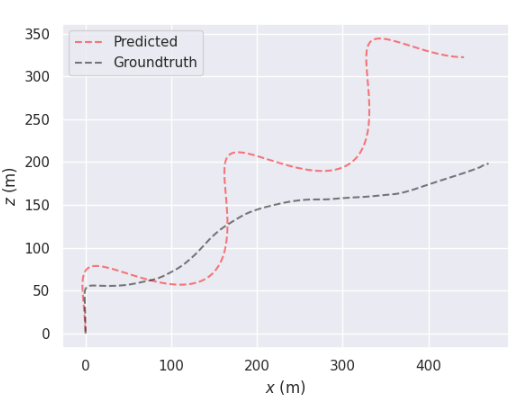
\includegraphics[width=0.8\textwidth]{./images/6_1_trajectory_3_encoder_only}
    \caption{Sequence 3 predicted by encoder-only model}
    \label{fig:trajectory-3-encoder-only}
\end{figure}

After a few trials with encoder-decoder model, which produced some circular trajectories, feeding the \textit{sequence 3} of KITTI (for more details \S~\ref{sec:kitti}) where the first pose of the sequence is considered as origin, we showed that the model (with both 6 and 12 layers of encoder-decoder) is able to learn a single sequence in over-fitting, but fails when trying to over-fit a more complex sequence.
The same model succeeded also in predicting the sequence 7, but failed when we combined the two sequences.
It also fails when we try to over-fit the most complicate sequence, the sequence 0.
\begin{figure}[H]
    \centering
    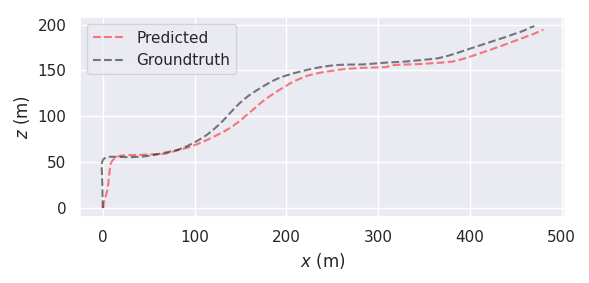
\includegraphics[width=0.8\textwidth]{images/6_1_well_predicted_seq_3}
    \caption{Good prediction sequence 3}\label{fig:well-predicted-seq-3}
\end{figure}
\begin{figure}[H]
    \centering
    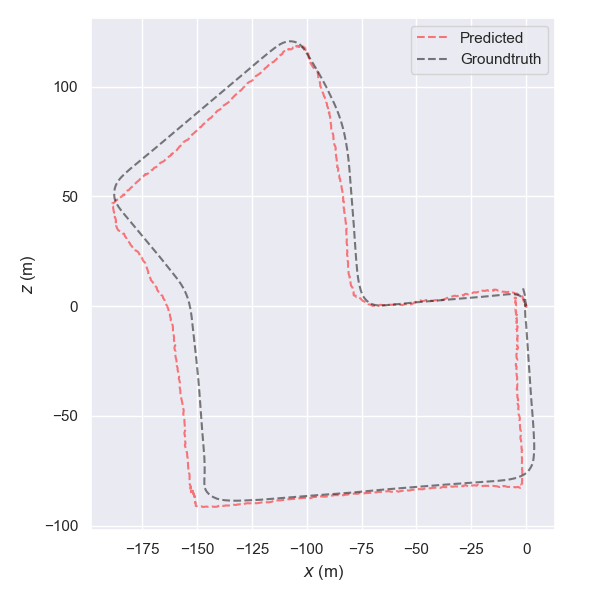
\includegraphics[width=0.8\textwidth]{images/6_1_well_predicted_seq_7}
    \caption{Good prediction sequence 7}\label{fig:well-predicted-seq-7}
\end{figure}
% %**************************************************************

\subsection{Autoregressive models}\label{subsec:autoregressive-model}
We implemented only the encoder-decoder version of the transformer in the autoregressive way, and most of the time the prediction of the network during the training on seq 3 is just a straight line.
So the model is \textbf{not} able to predict the simplest sequence in over-fitting.
The model could not predict any reasonable trajectory, predicting only a linear trajectory as the follow:
\begin{figure}[H]
    \centering
    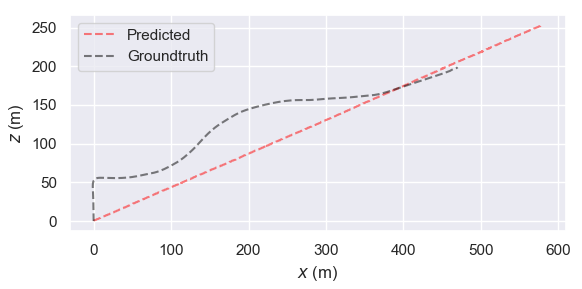
\includegraphics[width=0.8\textwidth]{images/6_1_autoregressive_prediction}
    \caption{Bad prediction sequence 3 of autoregressive model}\label{fig:autoregressive-seq-3}
\end{figure}
Although the model has been trained for more than two hundred epochs, the network cannot understand the goal, and this maybe is due to the loss function.

%**************************************************************

%\section{Knowledge acquired}\label{sec:knowledge-acquired}
By developing this project, I amplified my knowledge with various topics, such as:
\begin{itemize}
    \item Deep Learning,
    \item Computer Vision.
    \item Anaconda.
    \item PyTorch.
    \item Transformers.
    \item Auto-regressive models.
\end{itemize}
Especially, how the transformer works, and how to use it for computer vision tasks.
At the beginning of the project, the word ``transformer'' has had other meanings, but now, I know that it is a neural network architecture that is able to learn the sequence of images and the sequence of poses in a self-supervised way.
It's a general purpose architecture for domain adaptation from one sequence to another.
Another important notion that I learned is the concept of auto-regressive models.

To develop this approach, I had to deepen my knowledge about Visual Odometry, especially, a solid understanding of the task, basis knowledge such as the pose representations and the conversion between them.
I also had to amply my knowledge about the deep-learning framework, PyTorch, specifically, how to build a model, which are the components that are provided by the library, and how to use them.
For example, I had to implement the Transformer, initially I was implementing it from scratch, but then I discovered that there was some classes already implemented in the library, so I used latter ones, because they are more efficient and they are already tested.
I had to use Anaconda to manage the Python environment, because it is a very useful tool, and it is very easy to use.


%**************************************************************

\section{Future developments}\label{sec:future-developments}

During the training process, the loss function often converges to the minimum value at about 200 epoch.
But it does not decrease anymore, and the trajectory does not improve anymore.
So, we should use a different loss function instead of the one used, MSE o WSME, because they are not suitable for this task.
An ideal loss function for this task should describe the error in a way that the network can understand.

Another problem is that we do not have a large amount of data, so we should create synthetic dataset which is more suitable for this task.
For example, we can follow the approach adopted by Richter et al. (\cite{synthetic_dataset}), in this way we can create a dataset with a large number of images and poses.
Then, use it for pre-training, and finally, use the real KITTI dataset for fine-tuning.

We should also try with a different feature extractor, because the ResNets are designed for the classification task, and the embedding produced describes the image as whole, losing local information.
This is because the use of pooling layers, which are used to guarantee the translation invariance of the network when performing the classification or object detection tasks.
Meanwhile, for a task like VO this translation invariance is harmful, because it does not allow the network to learn the local features of the image.
The approach adopted by Dosovitsky et al. (\cite{vit_paper}), which consisted in split the image in smaller patches, then extract the embedding for each patch, and then combine them, could be a good solution.

Another experiment could be to change totally the feeding strategy, using a pair of images stacked together as did in many approaches, for example in ~\cite{deep_vo}.
In the same way, we can try to use the optical flow of the input images to help the network to understand the local motion.

As last attempt, it would be useful to try to use a RNN as prediction head, because it is able to learn the temporal information, and it can predict the next pose given the previous ones, also because, in the literature, good results have been reached using RNNs.

%**************************************************************

\section{Personal Evaluation}\label{sec:personal-evaluation}
By doing this project, I learned a new way-of-working and I improved my knowledge in various topics and fields.
I think this is very educational, and it introduced me into the world of research, letting me know that not every trial is successful, and that it is necessary to be meticulous and to have a lot of patience if you want to achieve good results.
I also learned that it is necessary to have a good knowledge of the topic, and to have a solid background, to do a lot of researches and to read a lot of papers, to understand the problem and to find the best solution.

It has been an interesting experience, and I think that I have learned a lot, improving my abilities to work with neural networks, to fix their problem and to see the results in a critical way.

Finally, I would like to thank my supervisor, Prof.~Luigi Di Stefano and my co-supervisor, Luca De Luigi for being so helpful and patient to help me to complete this project.
Without their help, I would not have been able to complete this project.

%**************************************************************

    %**************************************************************
    % Materiale finale
    %**************************************************************
    \backmatter
    \printglossaries
    % !TEX encoding = UTF-8
% !TEX TS-program = pdflatex
% !TEX root = ../tesi.tex

%**************************************************************
% Bibliografia
%**************************************************************

\cleardoublepage
% \chapter{Bibliopraphy}\label{ch:bibliografia}

\nocite{*}
% Stampa i riferimenti bibliografici
\printbibliography
%\printbibliography[heading=subbibliography,title={Bibliography references},type=book]

% Stampa i siti web consultati
%\printbibliography[heading=subbibliography,title={Website references},type=online]
%\printbibliography[heading=subbibliography,title={Paper references},type=article]


\end{document}
